\documentclass[12pt]{article}
\usepackage{preamble}

\pagestyle{fancy}
\fancyhead[LO,LE]{Физические основы компьютерных \\ и сетевых технологий}
\fancyhead[RO,RE]{Лекции Герта А. В.}

\fancyfoot[L]{\scriptsize исходники найдутся тут: \\ \url{https://github.com/pelmesh619/itmo_conspects} \Cat}

\renewcommand{\thesection}{}

\begin{document}

    \tableofcontents
    \clearpage

    % begin physics2_2025_02_10.tex





\section{Лекция 1. Магнитное поле}

Давным-давно верили, что существовал \enquote{эфир}, который опоясывал всю вселенную и который был посредником в гравитационных/электромагнитных 
взаимодействиях. Позднее от теории эфира перешли к теории поля. Согласно нее каждый электрический заряд создает электрическое поле, 
которое действует на другие заряды

Опыт показывает, что сила $\vec{F}$, действующая на точечный заряд $q$, зависит в общем случае не только от положения этого \
заряда, но и от его скорости $v$. Соответственно этому силу $F$ разделяют на две составляющие - электрическую $F_\text{Э}$ 
(не зависит от движения заряда) и магнитую $F_\text{М}$ (зависит от скорости заряда). В любой точке пространства направление и модуль
магнитной силы зависят от скорости $v$ заряда, причем эта сила всегда перпендикулярна вектору $v$. Свойства магнитной 
силы можно описать, если ввести понятие магнитного поля. Силовой характеристикой магнитного поля (его действия на двигающиеся заряженные частицы)
в данной точке пространства является вектор магнитной индукции $B$. Он определяет магнитную силу, действующую на двигающийся электрический заряд $q$

\[F_\text{М} = q [\vec{v}, \vec{B}]\]

Полная электромагнитная сила, действующая на заряд $q$: $F_L = q\vec{E} + q[\vec{v}, \vec{B}]$

Силу $F_L$ называеют силой Лоренца. Выражение выше справедливо как для постоянных, так и для переменных
электрических и магнитных полей при любых значениях скорости $v$ заряда. По действию силы Лоренца
на заряд можно в принципе определить модули и направления векторов $E$ и $B$. Поэтому выражение для силы Лоренца
можно рассматривать как определение электрического и магнитного полей

Магнитная часть силы Лоренца действует на движущийся заряд в направлении, перпендикулярном его скорости, и,
таким образом, не совершает работы над зарядом, оставляя неизменной его энергию и меняя лишь направление импульса
(изменяет траекторию движения частицы)

Магнитная сила не делает вклад в тангенциальную составляющую скорости, следовательно не изменяет энергию заряда и не делает работы

Магнитная часть силы Лоренца максимальна, если направление движения частицы составляет с направлением магнитного поля 
прямой угол, и равна нулю, если частица движется вдоль направления магнитного поля

Сила Лоренца не зависит от выбора системы отсчета, однако магнитная составляющая силы Лоренца меняется при переходе от одной
системы отсчета к другой (из-за изменения $v$).

Опыты показывают, что магнитное поле порождается движущимися зарядами. В результате обощения экспериментальных данных
был получен закон, определяющий поле $B$ точечного заряда $q$, движущегося с постоянной нерелятивистской скоростью $v$. 
Этот закон записывается в виде:

\[\vec{B} = \frac{\mu_0}{4\pi} \frac{q [\vec{v}, \vec{r}]}{r^3}\]

где $\mu_0$ - магнитная постоянная ($\frac{\mu_0}{4\pi} = 10^{-7} \frac{\text{Гн}}{\text{м}}$), $r$ - радиус-вектор, проведенный от заряда $q$ к точке наблюдения

Магнитная постоянная существует из-за СИ (в СГС $\mu_0 = 1$). В некоторых средах $\mu_0$ заменяется на $\mu_0 \mu$, где $\mu$ - магнитная проницаемость среды

\mediumvspace

Конец радиус-вектора $r$ неподвижен в данной системе отсчета, а его начало движется со скоростью $v$, поэтому
вектор $B$ в данной системе отсчета зависит не только от положения точки наблюдения, но и от времени

Пока что мы будем разбирать системы с равномерно двигающимися частицами

В соответствии с формулой вектор $B$ перпендикулярен плоскости, в которой расположены $v$ и $r$.
Единицей магнитной индукции служит тесла (Тл). Формулу можно представить как:

$\vec{B} = \frac{\mu_0}{4\pi} \frac{q [\vec{v}, \vec{r}]}{r^3} = \varepsilon_0 \mu_0 \left[\vec{v}, \frac{q}{4\pi\varepsilon_0} \frac{\vec{r}}{r}\right] = 
\varepsilon_0 \mu_0 [\vec{v}, \vec{E}] = \frac{[\vec{v}, \vec{E}]}{c^2}$, где $c = \frac{1}{\sqrt{\varepsilon_0 \mu_0}}$ - электродинамическая постоянная, равная скорости света в вакууме

Из этого следует, что магнитное поле не может быть без электрического поля

\mediumvspace

Для магнитного поля справедлив \textbf{принцип суперпозиции}: вектор магнитного поля в точке равен сумме магнитных полей,
создаваемых каждым зарядом или током в отдельности: $\vec{B} = \sum_i \vec{B}_i$

Найдем, пользуясь формулой магнитное поле, создаваемое постоянными электрическими токами. Подставим вместо $q$ заряд $dq = \rho dV$, где $dV$ - элементарный объем,
$\rho$ - объемная плотность заряда, и учтем, что $\rho v_d = j$ ($v_d$ - дрейфовая скорость носителей заряда (средняя скорость частиц)). 
Тогда формула получает такой вид: $d\vec{B} = \frac{\mu_0}{4\pi} \frac{[\vec{j}, \vec{r}] dV}{r^3}$

Если ток силы $I$ течет по тонкому проводу с площадью поперечного сечения $S$, то 

\[\vec{j} dV = S dl = Idl\]

\[\vec{j} dV = Id\vec{l}\]

Векторы $jdV$ и $Idl$ называют объемным и линейным элементами тока соответственно

Получам $\vec{B} = \frac{\mu_0}{4\pi} \int_l \frac{I[d\vec{l}, \vec{r}]}{r^3} = \frac{\mu_0}{4\pi} \int_V \frac{[\vec{j}, \vec{r}] dV}{r^3}$ - \textbf{Закон Био-Савара}

Расчет по этим формулам индукции магнитного поля тока значительно упрощается, если распределение тока имеет определенную симметрию

\begin{minipage}{\textwidth}
    \begin{wrapfigure}{R}{0pt}
        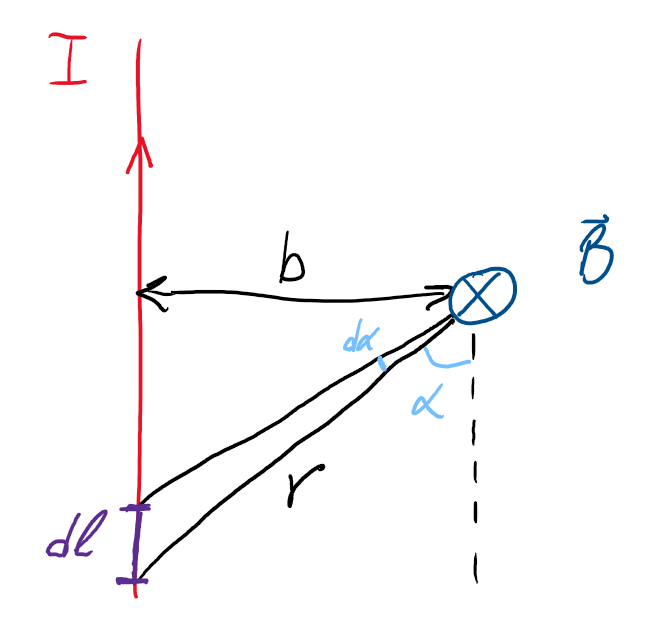
\includegraphics[width=5.8cm]{physics2/images/physics2_2025_02_10_2}
    \end{wrapfigure}

    \Ex Магнитное поле прямого тока, то есть тока, текущего по тонкому прямому проводу. Согласно формуле в произвольной точке $A$
    векторы $dB$ от всех элементов тока имеют одинаковое направление. Поэтому сложение векторов $dB$ можно заменить сложением 
    их модулей: $dB = \frac{Idl \cdot r \sin \alpha}{r^3} = \frac{\mu_0}{4\pi} I \frac{dl \sin\alpha}{r^2} =
    \frac{\mu_0}{4\pi} I \frac{r d\alpha}{r^2} = \frac{\mu_0}{4\pi} I \frac{d\alpha}{\frac{b}{\sin\alpha}} = \frac{\mu_0}{4\pi} \frac{I}{b} \sin \alpha d\alpha$, где $b$ - расстояние от точки до прямого проводника

    В интеграле получаем $B = \frac{\mu_0}{4\pi} \int_{0}^{\pi} \frac{I}{b} \sin \alpha d\alpha = \frac{\mu_0}{4\pi} \frac{I}{b} (\cos \alpha_1 - \cos \alpha_2)$

    Для бесконечного проводника получаем $B = \frac{\mu_0}{2\pi} \frac{I}{b}$
\end{minipage}

Линии магнитной индукции поля прямого тока представляют собой систему охватывающих провод концентрических окружностей

\begin{center}
    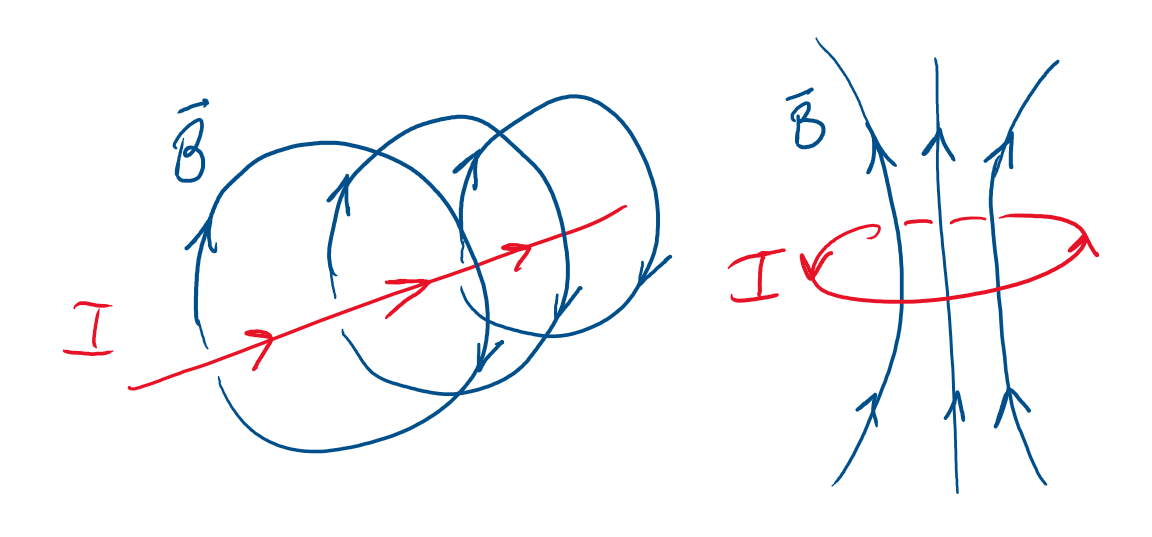
\includegraphics[width=0.7\textwidth]{physics2/images/physics2_2025_02_10_1}
\end{center}

Важно заметить, что линии электрического поля не замкнуты - у них есть начало (в плюсе) и конец (в минус), тогда 
как линии магнитного поля - замкнуты

\begin{minipage}{\textwidth}
    \begin{wrapfigure}{R}{0pt}
        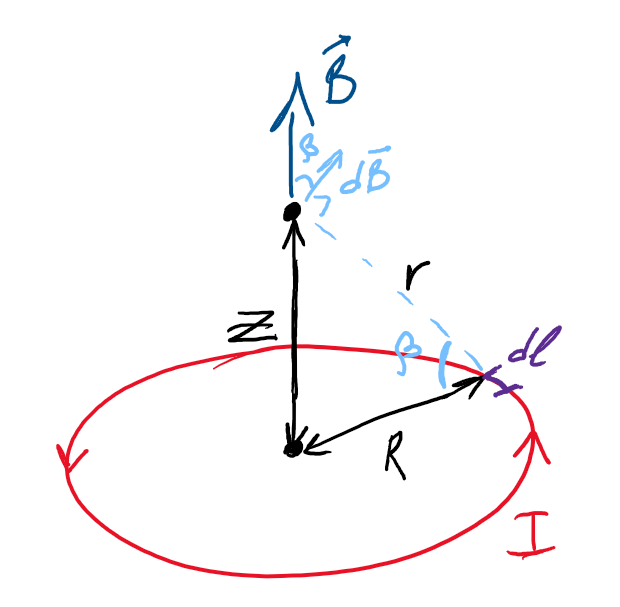
\includegraphics[width=5.8cm]{physics2/images/physics2_2025_02_10_3}
    \end{wrapfigure}

    \Ex Магнитное поле на оси кругового тока. Ищем вектор индукции в точке на оси кольца. 
    В силу симметрии вектор магнитной индукции сонаправлен оси кольца. По закону Био-Савара получаем

    $dB_z = dB \cos \beta = \frac{\mu_0}{4\pi} \frac{Idl \cdot r\sin 90^\circ}{r^3} \cos \beta$

    $\cos \beta = \frac{R}{r} \Longrightarrow B(z) = \frac{\mu_0}{4\pi} \frac{2\pi R^2 I}{(z^2 + R^2)^\frac{3}{2}} = \frac{\mu_0 R^2 I}{2 (z^2 + R^2)^\frac{3}{2}}$
\end{minipage}

\clearpage



% end physics2_2025_02_10.tex

% begin physics2_2025_02_17.tex





\section{Лекция 2. Теорема Гаусса для магнитного поля}

В электростатике было введено понятие потока вектора напряженности электрического поля. Аналлогичное понятие
можно ввести для магнитного поля. 

\Def Потоком вектора магнитной индукции (или магнитным потоком) через элемент
площади $dS$ называется скалярная величина, равная $d\Phi = \vec{B} d\vec{S} = B dS \cos \alpha = B_n dS$

Полный магнитный поток через поверхность $S$ равен сумме магнитных потоков через все элементы поверхности:

\[\Phi = \int_S \vec{B} d\vec{S}\]

Теорема Гаусса для вектора индукции магнитного поля: поток вектора магнитной индукции сквозь произвольную замкнутую
поверхность равен нулю:

\[\oint_S \vec{B} d\vec{S} = 0, \quad \mathrm{div}\vec{B} = 0\]

Эта теорема отражает факт непрерывности силовых линий магнитного поля, то есть отсутствия \enquote{магнитных зарядов}, 
на которых бы начинались или заканчивались линии магнитной индукции

Так как линии вектора индукции магнитного поля не имеют ни начала, ни конца, то число силовых линий, входящих в 
ограниченную замкнутую поверхность, равно числу выходящих из нее

Пусть магнитное поле создано бесконечно длинным прямолинейным проводником с током. Рассчитаем циркуляцию вектора
индукции магнитного поля по произвольному замкнутому контуру, охватывающему проводником

\[\oint_L \vec{B} d\vec{l} = \oint_L Bdl \cos\alpha\]

\[dl \cos \alpha = r d\varphi, B = \frac{\mu_0 I}{2\pi r} \Longrightarrow \oint_L \vec{B} d\vec{l} = \frac{\mu_0 I}{2\pi} \oint_L d\varphi = \mu_0 I\]

Получаем теорему о циркуляции вектора магнитной индукции: 

\begin{MyTheorem}
    Циркуляция вектора магнитной индукции по произвольному замкнутому
    контуру равна произведению магнитной постоянной на алгебраическую сумму токов, охватываемых этим контуром (или пронизывающих поверхность, опирающуюся на этот контур):

    \[\oint_L \vec{B} d\vec{l} = \mu_0 \sum_k I_k\]
\end{MyTheorem}

При вычислении суммы токов нужно учитывать знаки: положительными считаются те токи, направление которых связано с направлением обхода
контура правилом правого винта, отрицательными - токи противоположного направления

Если контур в проводящей среде с непрерывным распределением тока, то $\oint_L \vec{B} d\vec{l} = \mu_0 \int_S \vec{j} d\vec{S}$

По теореме Стокса: $\oint_L \vec{B} d\vec{l} = \int_S \mathrm{rot}\vec{B} d\vec{S} = \mu_0 \int_S \vec{j} d\vec{S}$

Таким образом, $\mathrm{rot}\vec{B} = \mu_0 \vec{j}$


\Ex Найдем магнитное поле соленоида (катушки)

Возьмем контур $L_1$ (см. кривой рисуночек), в нем $\oint_{L_1} \vec{B} d\vec{l} = (B_{23} - B_{41})l = 0 \Longrightarrow B_{23} = B_{41} = B_\text{внутри}$

В другом контур $L_2$ $\oint_{L_2} \vec{B} d\vec{l} = B_\text{внутри} l = \mu_0 NI \Longrightarrow B_\text{внутри} = \mu_0 \frac{N}{l} I = \mu_0 n I$, где $n$ - плотность витков катушки на длину катушки

\begin{center}
    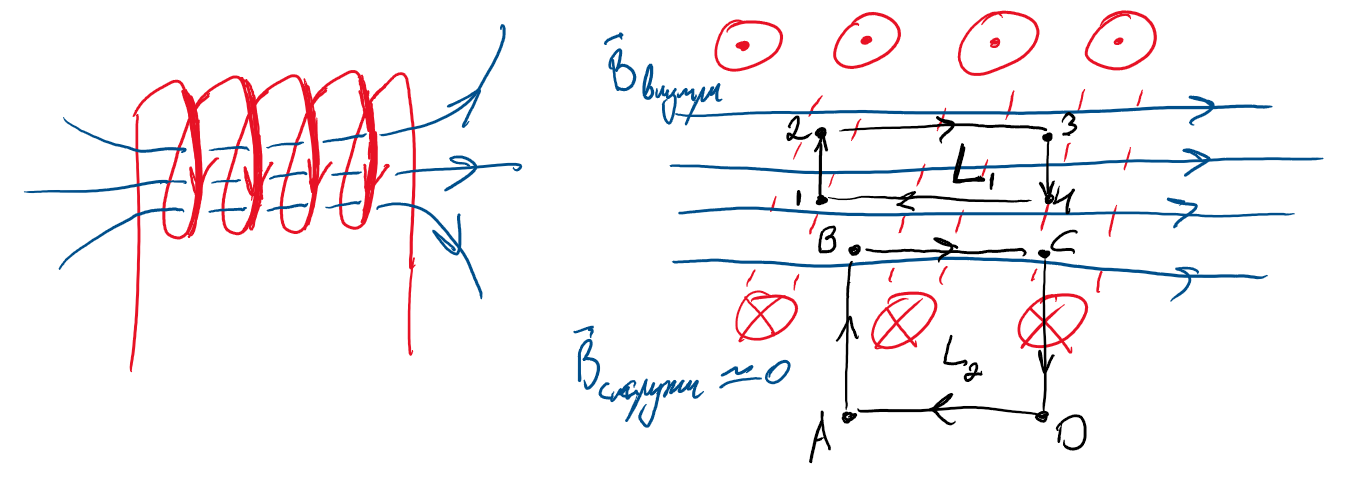
\includegraphics[width=15cm]{physics2/images/physics2_2025_02_17_1}
\end{center}

Получаем \fbox{$B = \mu_0 n I$} - поле катушки пропорционально плотности витков

\begin{minipage}{\textwidth}
    \begin{wrapfigure}{R}{0pt}
        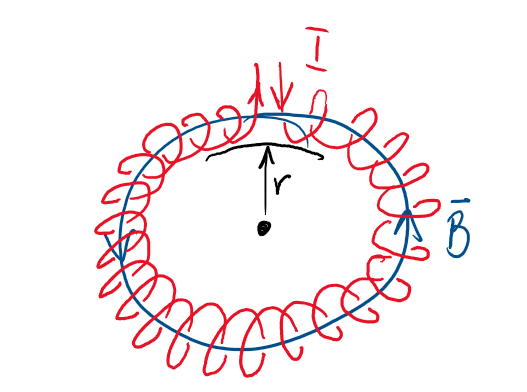
\includegraphics[width=6.3cm]{physics2/images/physics2_2025_02_17_2}
    \end{wrapfigure}

    \Ex Найдем поле тороида. Из соображений симметрии очевидно, что линии индукции - окружность, концентричные с тороидом. В качестве контура $L$ выберем окружность с радиусом $r$

    $\oint_L \vec{B} d\vec{l} = B \cdot 2\pi r = \mu_0 N I \Longrightarrow$ \fbox{$B(r) = \frac{\mu_0 N I}{2\pi r}$}, 
    где $N$ - число витков

    Вектора магнитной индукции будут являться касательными к окружности, концентричной тороиду

\end{minipage}

\Ex Постоянный ток $I = 10$ А, течет по длинному прямому проводнику круглого сечения. Найти магнитный поток через одну
из половин осевого сечения проводника в расчете на один метр его длины.

\mediumvspace

Возьмем контур $L$ - окружность радиуса $r$, меньшего радиуса сечения проводника $R$. 
По теореме о циркуляции $\oint_L B(r) dr = \mu_0 I_\text{внутри}$. В силу симметрии считаем, что вектор $\vec B(r)$ равен по модулю на всем контуре $L$.
Тогда получаем $B(r) \cdot 2\pi r = \mu_0 I_\text{внутри} = \mu_0 j S = \mu_0 j \pi r^2 \Longrightarrow B(r) = \frac{\mu_0 I r}{2 \pi R^2}$

Тогда поток через половину осевого сечения равен $\frac{\Phi}{l} = \int_0^R B(r) dr = \int_0^R \frac{\mu_0 I r}{2\pi R^2} dr = $ \fbox{$\frac{\mu_0 I}{4 \pi}$} $ = 10^{-6} \frac{\text{Вб}}{\text{м}}$

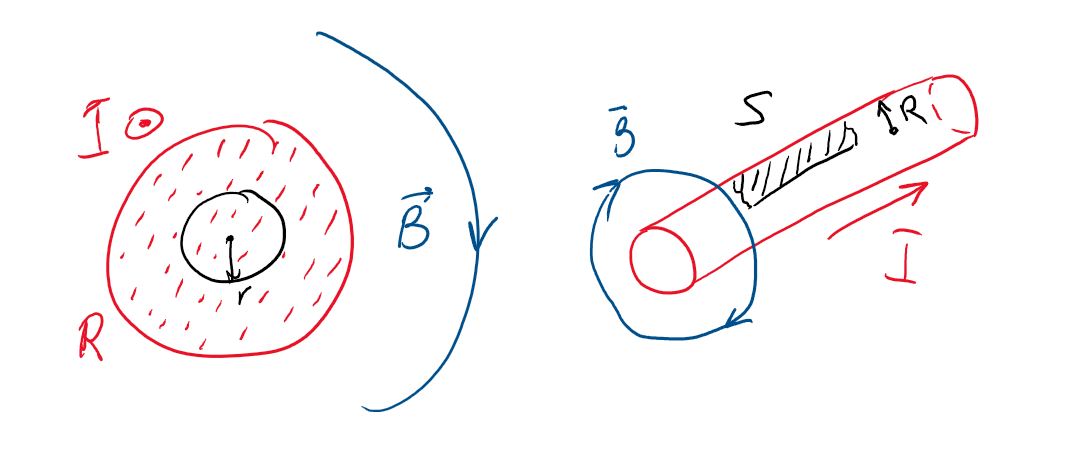
\includegraphics[width=15cm]{physics2/images/physics2_2025_02_17_3}

\begin{minipage}{\textwidth}
    \begin{wrapfigure}{R}{0pt}
        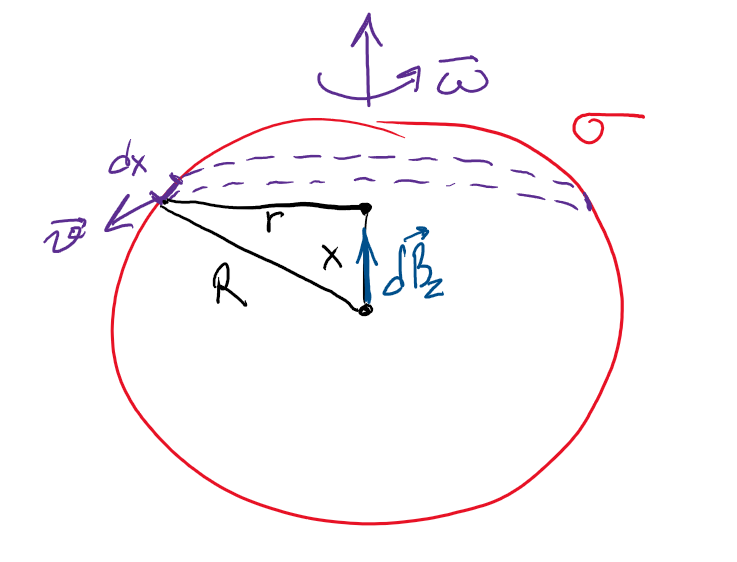
\includegraphics[width=6cm]{physics2/images/physics2_2025_02_17_4}
    \end{wrapfigure}

    \Ex Непроводящая сфера радиуса $R = 50$ мм, заряженная равномерно с поверхностной плотностью $\sigma = 10$ мкКл/м$^2$, 
    вращается с угловой скоростью $\omega = 70$ рад/с вокруг оси, проходящей через ее центр. Найти магнитную индукцию в центре сферы

    \mediumvspace

    Сделаем разбиение сферы на колечки высотой $dx$, длина каждой такой колечки равна $2\pi r$, где $r = \sqrt{R^2 - x^2}$.
    Его площадь $2\pi r dx$. Точка на кольце движется с линейной скоростью $v = \omega r$.
\end{minipage}

В силу симметрии вектор магнитной индукции $d\vec{B}$, производимый кольцом, параллелен оси $Oz$. 
Тогда $dB = \frac{\mu_0}{4\pi} \frac{q \cdot v}{R^2} = \frac{\mu_0}{4\pi} \frac{\sigma 2\pi r \cdot dx \cdot \omega r}{R^2} = 
\frac{\mu_0}{4\pi} \frac{\sigma 2\pi \omega (R^2 - x^2)}{R^2} dx$

В интеграле $B = \int_{-R}^R dB = \frac{\sigma \mu_0 \omega}{2} \int_{-R}^R \frac{(R^2 - x^2)}{R^2} dx = 
\frac{\sigma \mu_0 \omega}{2} \frac{(R^2 x - \frac{1}{3} x^3)}{R^2} \Big|_{-R}^R = 
\frac{\sigma \mu_0 \omega}{2} \frac{(R^2 x - \frac{1}{3} x^3)}{R^2} \Big|_{-R}^R = 
\frac{\sigma \mu_0 \omega}{2} \frac{4}{3} R = $ \fbox{$\frac{2}{3} \mu_0 R \omega \sigma$}

\clearpage


% end physics2_2025_02_17.tex

% begin physics2_2025_02_24.tex





\section{Лекция 3. Сила Ампера. Явление электромагнитной индукции}

\subsection{Сила Ампера}

Вектор магнитной индукции характеризует силовое действие магнитного поля на движущиеся заряды. 
Сила, действующая на движущийся точечный зарядв магнитном поле, равна $\vec{F}_{\text{Л (М)}} = q [\vec{v}, \vec{B}]$
и называется магнитной составляющей силы Лоренца

Направление магнитной составляющей силы Лоренца зависит от знака заряженной частицы

Магнитная составляющая силы Лоренца всегда направлена перпендикулярно скорости, поэтому не совершает работы и не изменяет величину скорости заряженной частицы

\begin{wrapfigure}{r}{0pt}
    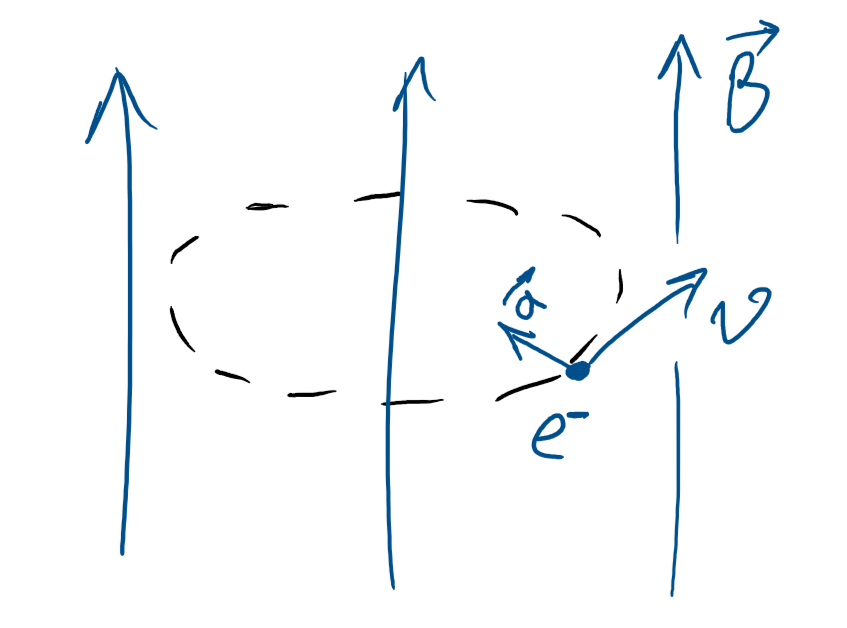
\includegraphics[width=6.2cm]{physics2/images/physics2_2025_02_24_1}
\end{wrapfigure}

\Ex Частица влетает перпендикулярно силовым линиям магнитного поля: $\vec{v} \perp \vec{B}$

Скорость частицы и действующая на нее сила все время лежат в плоскости, перпендикулярной к силовым линиям магнитного поля. 
Траекторией движения частицы будет окружность радиуса $R$, лежащая в этой плоскости. 
Условием движения по окружности является $q v B = m\frac{v^2}{R}$, из этого $R = \frac{mv}{qB}$


\Ex Частица влетает под углом $\alpha$ к силовым линиям магнитного поля

Составляющая скорости, направленная вдоль силовых линий магнитного поля, не будет изменяется, 
а в плоскости, перпендикулярной силовым линиям, частица движется по окружности. Траектория движения 
представляет собой винтовую линию

\Mem Сила Лоренца - полная сила, действующая на заряд: $\vec{F}_\text{Л} = q\vec{E} + q[\vec{v}, \vec{B}]$

Разделение полной силы Лоренца на электрическую и магнитную зависит от выбора системы отсчета

\Def Сила Ампера - сила, действующая под действием магнитного поля на заряды проводника, создающие электрический ток

Пусть электрический ток в объеме $dV$ элемента тока длиной $dl$ и площадью сечения $S$ образован заряженными частицами с зарядом
$q$, движущимися со средней скоростью $v$ вдоль элемента тока: 

\[d\vec{F}_A = [\vec{j}, \vec{B}] dV\]

\[d\vec{F}_A = I [d\vec{l}, \vec{B}]\]

Направление силы Ампера можно определить с помощью правила левой руки: если ладонь левой руки расположить так,
чтобы в нее входил вектор индукции магнитного поля, а четыре вытянутых - пальца по направлению тока, то отогнутый
на $90^\circ$ большой палец покажет направление силы Ампера

Для изучения свойств магнитного поля используется замкнутый плоский контур с током (рамка с током). Форма контура
не имеет значения, а его размеры должны быть малы по сравнению с расстоянием до источников магнитного поля.
Контур с током принято характеризовать магнитным моментом: $\vec{p}_m = I S \vec{n}$, где $I$ - сила тока, $S$ - площадь,
ограниченная контуром, $\vec{n}$ - нормаль, образующая с направлением тока правовинтовую систему

На контур с током действует сила Ампера $d\vec{F}_A = I[d\vec{l}, \vec{B}] \Longrightarrow \vec{F}_A = I \oint [d\vec{l}, \vec{B}]$

Если поле однородно, то $\vec{F}_A = I \oint [d\vec{l}, \vec{B}] = I [\oint d\vec{l}, \vec{B}] = 0$

Если поле неоднородно, то $\vec{F} = p_m \frac{\partial \vec{B}}{\partial n}$

\begin{wrapfigure}{r}{0pt}
    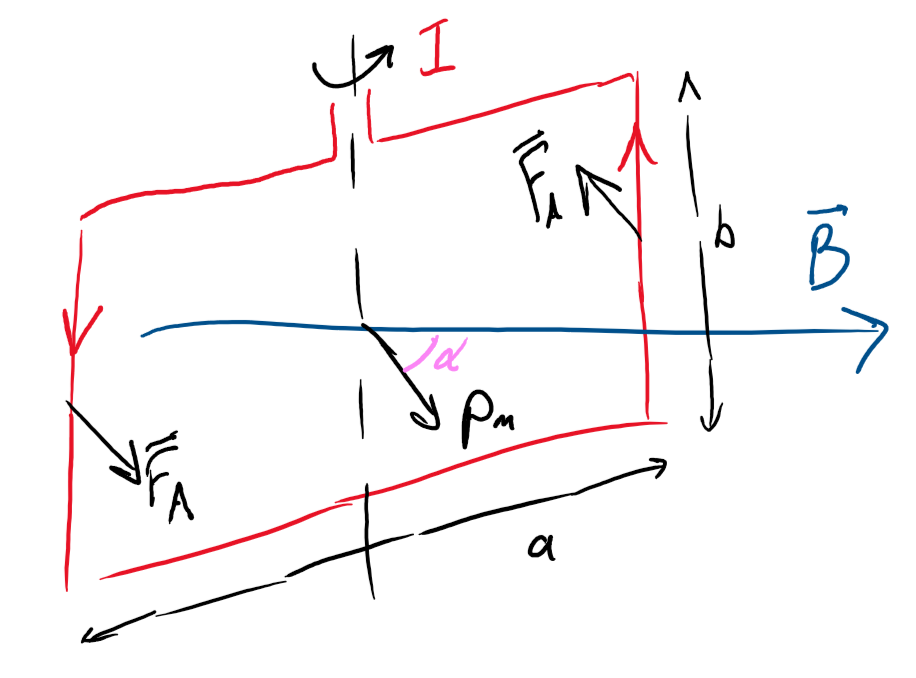
\includegraphics[width=7cm]{physics2/images/physics2_2025_02_24_2}
\end{wrapfigure}

\Ex Рассмотрим случай поведения прямоугольного контура с током в однородном магнитном поле. 
Предположим, что рамка имеет возможность вращаться вокруг оси, проходящей через середины ее
сторон длиной $a$ и перпендикулярной к силовым линиям магнитного поля.

Силы Ампера, действующие на стороны $a$ рамки, направлены вдоль оси вращения, 
поэтому действие этих сил сводится только к деформации контура (сжатию или растяжению).
Силы Ампера, действующие на стороны $b$ рамки, создают вращающий момент и равны $F_A = IBb$.

Тогда момент сил равен $M = F a \sin \alpha = I B S \sin \alpha = p_m B \sin \alpha \Longrightarrow \vec{M} = [\vec{p}_m, \vec{B}]$

\begin{wrapfigure}{r}{0pt}
    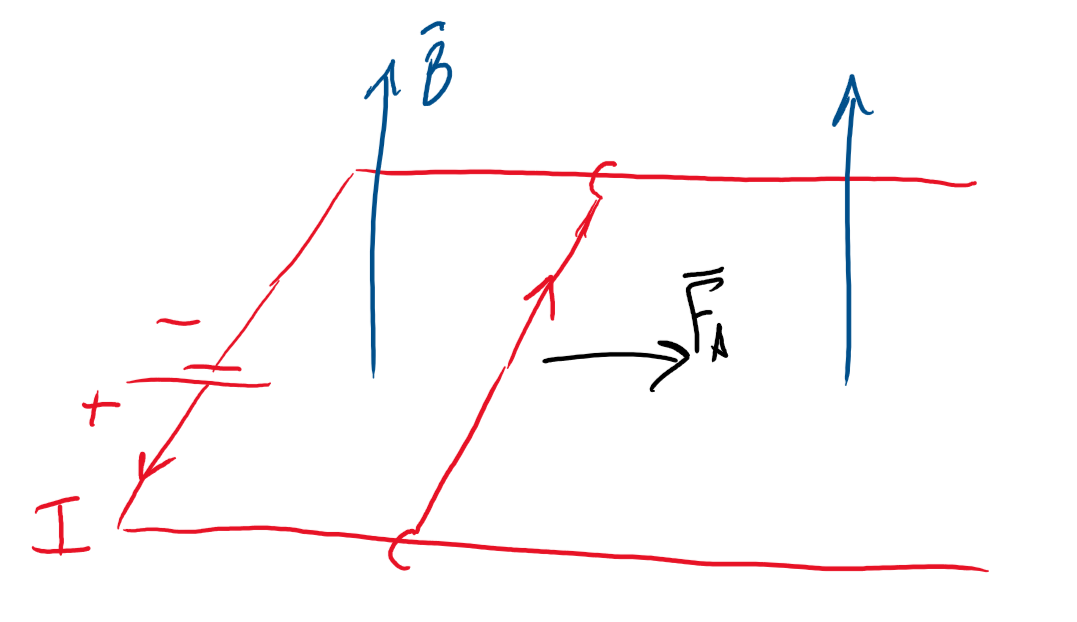
\includegraphics[width=7cm]{physics2/images/physics2_2025_02_24_3}
\end{wrapfigure}

\Ex Рассмотрим проводник в форме буквы \enquote{П} и двигающийся по нему другой проводник. 
По контуру, находящемуся в магнитном поле, течет ток, значит подвижный проводник будет двигаться влево, 
увеличивая площадь, охватываемого контуром. 

Работа сил магнитного поля по перемещению подвижного проводника будет равна:

$dA = d\vec{F} \cdot d\vec{r} = I [d\vec{l}, \vec{B}] \cdot d\vec{r} = Id\Phi$

$A = \int_1^2 Id\Phi$


\subsection{Явление электромагнитной индукции. Закон Фарадея. Правило Лоренца}

\begin{wrapfigure}{r}{0pt}
    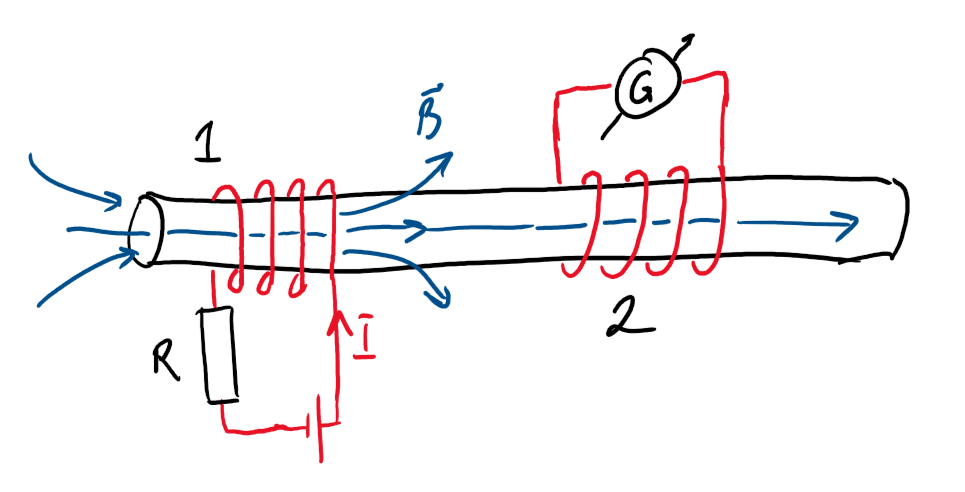
\includegraphics[width=6.2cm]{physics2/images/physics2_2025_02_24_4}
\end{wrapfigure}

В цепи первой катушки течет постоянный ток $I_1$, в цепи второй ток отсутствует. 
Если катушку 1 приближать к 2, в последней возникнет ток $I_2$, который Фарадей назвал индукционным током. 
При удалении катушки 1 от 2 ток $I_2$ тоже появляется, но имеет противоположное направление.

Катушку 1 можно заменить длинным полосовым магнитом. При перемещении магнита вдоль оси катушки 2, тоже обнаружится возникновение в ней 
индукционного тока.

Явление электромагнитной индукции заключается в возникновении электрического тока в замкнутом проводящем
контуре при изменении магнитного потока, охватываемого этим контуром. 

\begin{MyTheorem}
    Закон Фарадея: ЭДС индукции в контуре пропорциональна скорости изменения магнитного потока сквозь площадь, 
    ограниченную контуром:

    \[\varepsilon = - \frac{d\Phi}{dt}\]
\end{MyTheorem}

\begin{MyTheorem}
    Правило Ленца: индукционный ток всегда направлен так, что его магнитное поле противодействует причине, вызвавшей его появление
\end{MyTheorem}

Самоиндукцией называется явление возникновение ЭДС индукции в электрической цепи вследствие
изменения электрического тока в этой же цепи.

Заметим, что $B \sim I$ и $\Phi \sim B$ (в отсутствии ферромагнетиков). Тогда $\Phi \sim I$ или же $\Phi = LI$

Коэффициент пропорциональности $L$ называется индуктивностью контура. Индуктивность контура зависит от его размеров
и формы, магнитных свойств среды

При изменении силы тока в контуре возникает ЭДС самоиндукции $\varepsilon_s = -\frac{d\Phi}{dt} = -\frac{d}{dt}(LI) = -L\frac{dI}{dt} - I\frac{dL}{dt}$

\clearpage

% end physics2_2025_02_24.tex

% begin physics2_2025_03_03.tex






\section{Лекция 4. Электромагнитная индукция и магнетики}

\subsection{Электромагнитная индукция}

Закон Фарадея связывает ЭДС индукции с изменением магнитного потока через контур:

\[
    \varepsilon_{\text{инд}} = \oint \vec{E} \cdot d\vec{l} = -\frac{\partial \Phi}{\partial t},
\]

где магнитный поток $\Phi = \int_S \vec{B} \cdot d\vec{S}$. 
Переменное магнитное поле создаёт вихревое электрическое поле: 
силовые линии такого поля замкнуты, а само поле действует на заряды даже в отсутствие проводника. 
Это явление лежит в основе работы трансформаторов и генераторов. 
Например, если быстро вращать магнит рядом с катушкой, возникающая ЭДС заставляет ток течь в цепи.

Для произвольного контура изменение потока связано с локальным изменением $\vec{B}$:

\[
    \frac{\partial \Phi}{\partial t} = \int_S \frac{\partial \vec{B}}{\partial t} \cdot d\vec{S}.
\]

ЭДС можно выразить через интеграл от производной магнитного поля:

\[
    \varepsilon_S = -\int_S \frac{\partial \vec{B}}{\partial t} \cdot d\vec{S}.
\]

Это означает, что чем быстрее меняется магнитное поле или чем больше площадь контура, 
тем сильнее индуцированный ток.

\subsection{Магнитное поле в веществе}

В материальной среде полное поле $\vec{B}$ складывается из внешнего $\vec{B}_0$ и поля $\vec{B}'$, 
создаваемого намагниченностью вещества. Магнитные свойства описываются вектором намагниченности $\vec{J}$ - 
магнитным моментом единицы объема:

\[
    \vec{J} = n\vec{p}_m, \quad [\vec{J}] = \text{А/м},
\]


где $n$ — концентрация атомов, $\vec{p}_m$ — магнитный момент одного атома. Намагниченность связана с молекулярными токами: каждый атом ведёт себя как микроскопический виток с током $I' = \vec{J} \cdot \vec{l}$ (рис. 1). Суммарный молекулярный ток через поверхность $S$ равен циркуляции $\vec{J}$ по контуру:

\[
    I' = \oint \vec{J} \cdot d\vec{l}.
\]

\vspace{0.5cm}

\noindent\textbf{Основные уравнения.} Полный ток (внешний $I$ и молекулярный $I'$) создаёт магнитное поле:

\[
    \oint \vec{B} \cdot d\vec{l} = \mu_0(I + I').
\]

Чтобы исключить молекулярные токи, вводят \textbf{напряжённость магнитного поля} $\vec{H}$:

\[
    \vec{H} = \frac{\vec{B}}{\mu_0} - \vec{J}, \quad \oint \vec{H} \cdot d\vec{l} = I.
\]

В дифференциальной форме: $\nabla \times \vec{H} = \vec{j}$, где $\vec{j}$ — плотность внешних токов. 
Для большинства веществ $\vec{B}$ и $\vec{H}$ связаны линейно:

\[
    \vec{B} = \mu_0\mu\vec{H}, \quad \vec{J} = \chi\vec{H},
\]

где $\mu = 1 + \chi$ — относительная магнитная проницаемость, $\chi$ — магнитная восприимчивость. 

\vspace{0.5cm}

\noindent\textbf{Граничные условия.} По аналогии с электрическим полем при переходе между средами с 
разными коэффициентами магнитной проницаемости:

\begin{itemize}
    \item Нормальная компонента $B$ непрерывна: $B_{1n} = B_{2n}$ (магнитные заряды не существуют).
    \item Касательная компонента $H$ скачкообразно меняется при наличии поверхностных токов: $H_{2\tau} - H_{1\tau} = I_{\text{пов}}$. 
    Если токов нет, $H_{1\tau} = H_{2\tau}$, 
    а $B$-поле меняется пропорционально $\mu$: $B_{2\tau} = \frac{\mu_2}{\mu_1} B_{1\tau}$.
\end{itemize}

\subsection{Типы магнетиков и энергия поля}

\noindent\textbf{Диамагнетики} (медь, вода) слабо выталкиваются из поля ($\chi < 0$, $|\chi| \sim 10^{-5}$). 
Их атомы не имеют собственного момента; наведённые токи ослабляют внешнее поле. 

\textbf{Парамагнетики} (алюминий) слабо втягиваются ($\chi > 0$, $\chi \sim 10^{-3}$): 
тепловое движение мешает ориентации атомных моментов. 

\textbf{Ферромагнетики} (железо) сильно усиливают поле ($\mu \gg 1$) за счёт доменов - 
областей спонтанной намагниченности. При циклическом перемагничивании наблюдается гистерезис: 
зависимость $B(H)$ образует петлю, что приводит к потерям энергии.

\vspace{0.5cm}

\noindent\textbf{Энергия магнитного поля.} При изменении тока в катушке совершается работа против ЭДС индукции:

\[
    dW = I \cdot d\Phi = L I \, dI \quad \Rightarrow \quad W = \frac{LI^2}{2}.
\]

Эта энергия «запасена» в поле: плотность энергии $w = \frac{B^2}{2\mu_0\mu}$. 
В ферромагнетиках часть энергии тратится на переориентацию доменов (гистерезисные потери).

% end physics2_2025_03_03.tex

% begin physics2_2025_03_10.tex





\section{Лекция 5. Колебания}

Колебаниями называются процессы (изменения состояния тела или системы), 
обладающие той или иной степенью повторяемости во времени. 
Повторение может быть строго периодическим (например, движение маятника) 
или хаотическим (апериодические колебания). Различают:

\begin{itemize}
    \item \textbf{Периодические:} значения физических величин повторяются через равные интервалы времени $T$
    
    \item \textbf{Апериодические:} нет строгой периодичности, например, затухающие колебания груза

    \item \textbf{Свободные (собственные):} возникают после выведения системы из равновесия \textit{без внешнего воздействия}
    
    \item \textbf{Вынужденные:} поддерживаются внешней периодической силой. Амплитуда зависит от соотношения частоты силы и собственной частоты системы (явление резонанса).
    
    \item \textbf{Автоколебания:} энергия поступает в систему по её внутренним законам. Пример: генератор на транзисторе, где обратная связь поддерживает незатухающие колебания.
\end{itemize}

Колебательная система - физическая система, в которой могут существовать свободные колебания. 
Реальные системы всегда имеют затухание из-за диссипативных сил (трение, сопротивление).
Систему, в которой описывающие ее величины совершают колебания около точки равновесия, называют осциллятором

Системы, в которых возможны колебательные процессы, подразделяются на линейные и нелинейные.
В первом случае дифференциальные уравнения, описывающие поведение системы, являются линейными, 
и система подчиняется принципу суперпозиции.

Во втором случае такие дифференциальные уравнения нелинейны и принцип суперпозиции не справедлив. Большинство
физических систем нелинейны, однако, при малых отклонениях от состояний равновесия они демонстрируют линейное поведение

\mediumvspace

Простейшими являются гармонические колебания, которые описываются формулой $x = A \cos (\omega_0 t + \alpha)$ 
(или $x = A \sin (\omega_0 t + \alpha)$). Обычно точка $x = 0$ считается положением равновесия. 

Такие колебания часто встречаются в природе (например, маятник). К тому же, другие периодические процессы 
могут быть представлены как комбинация гармонических (подобно рядам Фурье)

Величина $\alpha$ называется начальной фазой колебаний, а $A$ - амплитуда, наибольшее значение колебания. 
Косинус - $2\pi$-периодичная функция, из этого можно найти период колебаний: $(\omega_0 (t + T) + \alpha) - (\omega_0 t + \alpha) = 2\pi \Longrightarrow T = \frac{2\pi}{\omega_0}$

Период отражает величину времени, через которое система придет в исходное положение. Обратная величина - частота $\nu = \frac{1}{T}$

Можем получить скорость колебаний: $v_x = \dot x = -A \omega_0 \sin (\omega_0 t + \alpha)$

И ускорение: $a_x = \ddot x = -A \omega_0^2 \cos (\omega_0 t + \alpha)$

Из этого $\ddot x + \omega_0^2 x = 0$

По формуле Эйлера функцию гармонических колебаний можно представить как $x(t) = \operatorname{Re} (Ae^{i(\omega_0 t + \alpha)})$

\ExN{Пружинный маятник} Сила упругости по закону Гука равна $F = -kx$. Подставляя в $F = m\ddot{x}$, получаем:

\[
m\ddot{x} + kx = 0 \quad \Longrightarrow \quad \omega_0 = \sqrt{\frac{k}{m}}, \quad T = 2\pi\sqrt{\frac{m}{k}}
\]

Полная энергия в отсутствие трения сохраняется:$W = \frac{mv^2}{2} + \frac{kx^2}{2}$.
И в пике достигает $W_{\text{пот}} = W_{\text{кин}} = \frac{mv^2}{2} = \frac{mA^2\omega_0^2}{2} = \frac{kA^2}{2}$
    
\ExN{Математический маятник} - подвешенный грузик на нерастяжимой нити, совершающий движение по окружности.
Момент силы равет $M = m g l \sin \varphi, I = m l^2$, угловое ускорение - $\varepsilon = \frac{d^2 \varphi}{d t^2}$

По основному уравнению вращательного движения $I \varepsilon = M \Longrightarrow \ddot \varphi l = g \sin \varphi$

При малых колебаниях $\sin \varphi \sim \varphi$ и получаем $\varphi = \varphi_{\max} \cos (\omega_0 t + \alpha)$

Отсюда период $T = 2\pi\sqrt{\frac{l}{g}}, \omega_0 = \sqrt{\frac{g}{l}}$

\ExN{Электрический $LC$-контур:} 
Пусть конденсатор ёмкостью $C$ заряжен до напряжения $U_0$. 
При соединении конденсатора с катушкой индуктивности в цепи потечёт ток $I$, 
что вызовет в катушке ЭДС самоиндукции, направленную на уменьшение тока в цепи. 
Ток, вызванный этой ЭДС (при отсутствии потерь в индуктивности), 
в начальный момент будет равен току разряда конденсатора, то есть результирующий ток будет равен нулю. 
Магнитная энергия катушки в этот (начальный) момент равна нулю.

Затем результирующий ток в цепи будет возрастать, а энергия из конденсатора будет переходить 
в катушку до полного разряда конденсатора. В этот момент электрическая энергия конденсатора равна нулю. 
Магнитная же энергия, сосредоточенная в катушке, напротив, максимальна

После этого начнётся перезарядка конденсатора, то есть зарядка конденсатора напряжением другой полярности. 
Перезарядка будет проходить до тех пор, пока магнитная энергия катушки не перейдёт в электрическую энергию 
конденсатора. Конденсатор в этом случае снова будет заряжен до напряжения $-U_0$

\[
L\frac{d^2q}{dt^2} + \frac{q}{C} = 0 \quad \Longrightarrow \quad \ddot{q} + \frac{1}{LC}q = 0
\]

Отсюда циклическая частота: $\omega_0 = \frac{1}{\sqrt{LC}}$, период - $T = 2\pi\sqrt{LC}$

Энергия переходит между конденсатором $\left(W_E = \frac{q^2}{2C}\right)$ и катушкой $\left(W_M = \frac{LI^2}{2}\right)$.



% end physics2_2025_03_10.tex

% begin physics2_2025_03_17.tex





\section{Лекция 6. Колебания}

$T = 2\pi \sqrt{LC}$ - формула Томпсона

Напряжение на конденсаторе меняется в такт с зарядом

$U_C(t) = \frac{q}{C} = \frac{q_{\max}}{C} \cos (\omega_0 t + \alpha) = U_{\max} \cos (\omega_0 t + \alpha)$

А сила тока опережает по фазе напряжение на конденсаторе на $\frac{\pi}{2}$

$I(t) = \frac{dq}{dt} = -\omega_0 q_{\max} \sin(\omega_0 t + \alpha) = I_{\max} \cos(\omega_0 t + \alpha + \frac{\pi}{2})$


$U_{\max} = \frac{1}{\omega_0 C} I_{\max} = \sqrt{\frac{L}{C}} I_{\max}$

$W_E = \frac{C U^2_C (t)}{2}$

$W_B = \frac{L I^2(t)}{2}$

\subsection{Вектор колебаний}

Сложение нескольких гармонических колебаний одного направления и одинаковой частоты облегчается, 
если изображать колебания графически в виде векторов на плоскости. Полученная таким способом схема называется 
векторной диаграммой.

% https://www.geogebra.org/calculator/jhshxnfd

\begin{wrapfigure}{R}{0pt}
    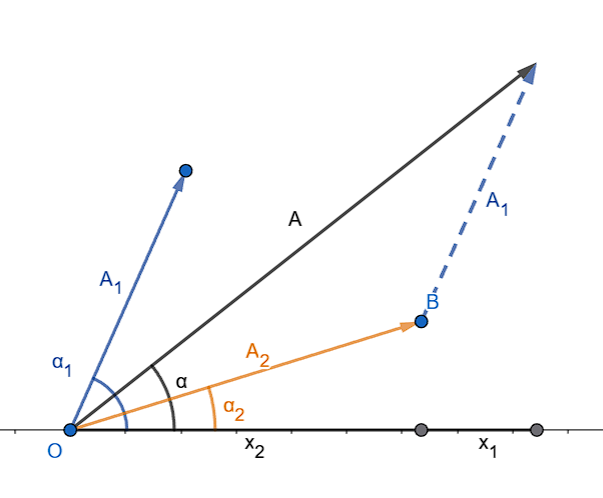
\includegraphics[width=6cm]{physics2/images/physics2_2025_03_17_1}
\end{wrapfigure}

Возьмем ось $Ox$, точку $O$, от оси с углом $\alpha$ отложим вектор длиной $A$. Если привести вектор
во вращение с угловой скоростью $\omega_0$, то проекция вектора будет перемещаться в по оси $Ox$ 
в пределах от $-A$ до $A$. Причем координата проекции будет изменяться по закону: $x(t) = A\cos (\omega_0 t + \alpha)$

Если два колебания представить с помощью векторов $A_1$ и $A_2$, то проекция суммы векторов $A$ на ось будет 
представлять сумму проекций. $A$ будет вращаться с той же частотой, что и $A_1$ и $A_2$

По геометрическим соображениям тангенс угла вектора $A$ $\alpha$ (также начальная фаза колебаний) равен 
$\tg \alpha = \frac{A_1 \sin \alpha_1 + A_2 \sin \alpha_2}{A_1 \cos \alpha_1 + A_2 \cos \alpha_2}$

Если частоты двух гармонических колебаний различны, то их сумма не будет являться гармоническим колебанием.
Но если колебания одного направления мало отличаются по частоте, то сумму колебаний можно рассматривать
как гармоническое колебание с пульсирующей амплитудой. Такое колебание называется биениями.

Рассмотрим одно колебание с частотой $\omega$, другое колебание с частотой $\omega + \Delta \omega$, причем $\Delta \omega \ll \omega$

Тогда $x = x_1 + x_2 = A (\cos \omega t + \cos ((\omega + \Delta \omega) t)) = 2 A \cos \frac{\Delta \omega}{2} \cdot 
\cos \left(\omega + \frac{\Delta \omega}{2}\right) t $

Величину $2 A \cos \frac{\Delta \omega}{2}$ можно рассматривать как амплитуду

% https://www.geogebra.org/calculator/cmxkpn3n

\begin{center}
    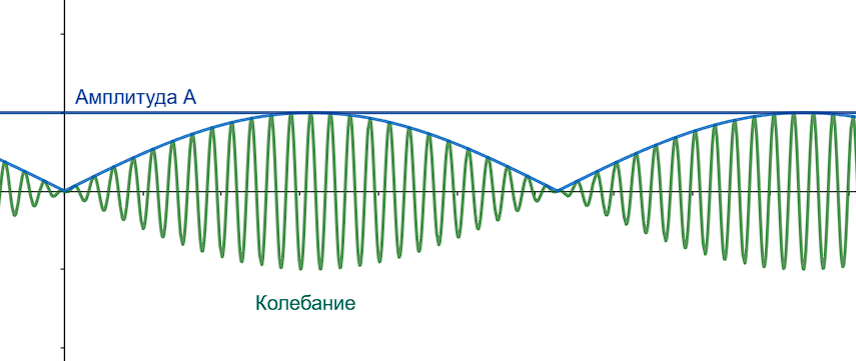
\includegraphics[width=13cm]{physics2/images/physics2_2025_03_17_2}
\end{center}

Предположим, что имеются две взаимно перпендикулярные векторные величины $x$ и $y$, изменяющиеся по закону:
$\vec x = \vec e_x A \cos \omega t, \qquad \vec y = \vec e_y B \cos (\omega t + \alpha)$

Здесь $e_x, e_y$ - орты координатных осей, $A, B$ - амплитуды

$\cos \omega t = \frac{x}{A}, \qquad \sin \omega t = \pm \sqrt{1 - \frac{x^2}{A^2}}$

$\frac{y}{B} = \cos (\omega t + \alpha) = \cos \omega t \cdot \cos \alpha - \sin \omega t \cdot \sin \alpha = 
\frac{x}{A} \cos \alpha \mp \sin \alpha \cdot \sqrt{1 - \frac{x^2}{A^2}}$

Немного преобразив выражение, получаем уравнение эллипса: $\frac{x^2}{A^2} + \frac{y^2}{B^2} - \frac{2xy}{AB} \cos \alpha = \sin^2 \alpha$

При $\alpha = 0$ результирующее движение является гармоническим колебанием вдоль прямой $y = \frac{B}{A} x$,
при других - эллипсом

% картинка 

При почти одинаковых частотах движение происходит по видоизменяющейся кривой. При разных частотах получаются фигуры Лиссажу

\subsection{Затухающие колебания}

Во всякой реальной колебательной системе всегда имеется либо сила трения, либо активное электрическое сопротивление,
действие которых приводит к уменьшению энергии системы 

Для пружинного маятника в вязкой среде получаем $m \ddot x = -kx - r\dot x$ или $\ddot x + 2 \beta \dot x + \omega^2_0 x = 0$

Ища решения в виде $x(t) = u(t) e^{\beta t}$, получаем $\ddot u + (\omega^2_0 - \beta^2) u = 0$

При $\omega_0 > \beta$ получим $\omega \equiv \sqrt{\omega^2 - \beta^2}$ и $\ddot u + \omega^2 u = 0$

Из этого $u = A_0 \cos (\omega t + \alpha)$, а $x(t) = A_0 e^{\beta t} \cos (\omega t + \alpha)$

Скорость затухания колебаний определяется величиной $\beta$, которую называют коэффициентом затухания. 
Также затухания можно характеризовать декрементом затухания $\lambda = \ln \frac{A(t)}{A(t + T)} = \beta T$

За время $\tau = \frac{T}{\lambda}$, за которое амплитуда уменьшается в $e$ раз, система успевает совершить $N_\tau = \frac{\tau}{T}$
колебаний

Также применяется величина добротности колебательной системы $Q = \frac{\pi}{\lambda}$

В электрическом колебательном контуре получаем $2\beta \equiv \frac{R}{L}$ и $\omega_0^2 \equiv \frac{1}{LC}$

$\ddot q + 2\beta \dot q + \omega^2_0 q = 0$

Здесь $\lambda = \frac{R}{2L} \cdot \frac{2\pi}{\omega} = \frac{R\pi}{L \omega}$, $Q = \frac{L\omega}{R}$


\subsection{Вынужденные колебания}

Пусть механическая колебательная система подвергается действию
внешней силы, изменяющейся со временем по гармоническому закону: $F_x = F_0 \cos \omega t$

Тогда $m\ddot{x} + r\dot{x} + kx = F_0 \cos(\omega t)$

Установившееся решение: $x(t) = \frac{F_0}{\sqrt{(k - m\omega^2)^2 + (r\omega)^2}} \cos(\omega t - \phi)$,
где $\phi = \arctan\left(\frac{r\omega}{k - m\omega^2}\right)$ — сдвиг фазы. 

Резонанс возникает при частоте: $\omega_{\text{рез}} = \sqrt{\omega_0^2 - 2\beta^2}$

Добротность определяет остроту резонанса: $Q = \frac{\omega_0}{2\beta}$.

% end physics2_2025_03_17.tex

% begin physics2_2025_03_24.tex





\section{Лекция 7. Электромагнитные волны}

Вспомним знаменитые уравнения Максвелла

\begin{itemize}
    \item $[\vec \nabla \vec E] = -\frac{\partial \vec B}{\partial t}$ - закон Фарадея

    \item $[\vec \nabla \vec D] = \rho$ - теорема Гаусса

    \item $[\vec \nabla \vec H] = \vec j + \frac{\partial \vec D}{\partial t}$ - закон Ампера

    \item $\vec \nabla \vec B = 0$ - теорема Гаусса для магнитного поля
\end{itemize}

А также $\vec \nabla \vec j = -\frac{\partial \rho}{\partial t}$ - уравнение непрерывности, $\vec B = \mu \mu_0 \vec H$, $\vec D = \varepsilon \varepsilon_0 \vec E$

В среде однородной, нейтральной ($\rho = 0$) и непроводящей ($j = 0$) получаем:

\begin{multicols}{2}
    \begin{center}
        $[\vec \nabla \vec E] = -\frac{\partial \vec B}{\partial t}$

        $[\vec \nabla \vec D] = 0$

        $[\vec \nabla \vec H] = \frac{\partial \vec D}{\partial t}$

        $\vec \nabla \vec B = 0$
    \end{center}
\end{multicols}

\mediumvspace

Из этого:

$\underset{\|}{\frac{\partial}{\partial t} \left(\frac{\partial \vec D}{\partial t}\right)} = \varepsilon \varepsilon_0 \frac{\partial^2 \vec E}{\partial t^2}$

$\frac{\partial}{\partial t} [\vec \nabla \vec H] = \left[\vec \nabla \frac{\partial \vec H}{\partial t}\right] = 
- \frac{1}{\mu \mu_0} [\vec \nabla [\vec \nabla \vec E]] = \vec \nabla (\vec \nabla \vec E) - (\vec \nabla \vec \nabla) \vec E 
\underset{\vec \nabla \vec D = \vec \nabla \varepsilon \varepsilon_0 \vec E = 0}{=\joinrel=\joinrel=} -\vec \nabla^2 \vec E$

Далее получаем $-\vec \nabla^2 \vec E = \varepsilon \varepsilon_0 \frac{\partial^2 \vec E}{\partial t^2}$. 
Приходим к волновым уравнениям: 

\begin{center}
    $\nabla^2 \vec E - \varepsilon \varepsilon_0 \mu \mu_0 \frac{\partial^2 \vec E}{\partial t^2} = 0$

    $\nabla^2 \vec H - \varepsilon \varepsilon_0 \mu \mu_0 \frac{\partial^2 \vec H}{\partial t^2} = 0$
\end{center}

Коэффициент перед вторым членом определяет скорость волны $v = \frac{1}{\sqrt{\varepsilon \varepsilon_0 \mu \mu_0}} = \frac{c}{\sqrt{\varepsilon \mu}}$, где $c$ - скорость света в вакууме

Главное отличие волны от колебания - это то, что волна переносит энергию

В простейшем случае решением уравнения может быть такая функция (так называемая гармоническая расходящася сферическая волна):

$E(\ver r, t) = E_0 \cos (\omega t \pm \vec k \vec r + \varphi_0)$, где $\vec k$ - волновой вектор, а $\vec r$ - расстояние от наблюдаемой нами точки до источника волн

В таком случае поток по сферам разных радиусов в центре источника будет одинаков

Если волна зависит только от одной координаты, то волна будет называться плоской: $E(x, t) = E_0 \cos (\omega t \pm k x + \varphi_0)$

Анализ электромагнитных волн (ЭМВ) показывает, что они обладают свойствами:

\begin{itemize}
    \item Вектора $\vec E$, $\vec B$ и $\vec k$ взаимно ортогональны и образуют правовинтовую тройку векторов
    \item Между напряженностью электрического поля и индукцией магнитного поля волны в вакууме существует прямая связь:
    $|\vec E| = c |\vec B|$ (не в вакууме $\sqrt{\varepsilon \varepsilon_0} |\vec E| = \sqrt{\mu \mu_0} |\vec B|$)
\end{itemize}

При этом начальная фаза и частота у колебаний $B$ и $E$ равны

Объемная плотность ЭМ-энергии равна: $w = \frac{\varepsilon \varepsilon_0 E^2}{2} + \frac{\mu \mu_0 H^2}{2}$. 
Из этого $w = \varepsilon \varepsilon_0 E^2 = \mu \mu_0 H^2 = \frac{EH}{v}$, где $v$ - скорость волны

Вектор $\vec S = [\vec E \vec H]$ называют вектором Умова-Пойнтинга и отображает плотность потока энергии 

Интенсивность волны (мощность, переносимая через площадку за время) равна усредненному модулю вектора Умова-Пойнтинга за данный промежуток времени $I = \Pair{|\vec S|} = \frac{1}{2} \sqrt{\frac{\varepsilon \varepsilon_0}{\mu \mu_0}} E^2_m$

Для ЭМВ также справедлив эффект Доплера:

\begin{itemize}
    \item Продольный: $f = f_0 \cdot \sqrt{\frac{1 - \frac{v}{c}}{1 + \frac{v}{c}}}$

    \item Поперечный: $f = f_0 \cdot \sqrt{1 - \frac{v^2}{c^2}}$
\end{itemize}

Здесь $f_0$ - частота волн, испускаемых источником, $f$ - частота волн, воспринимаемых приемников, $v$ - скорость источника относительно приемника

Из граничных условий при переходе между средами и из знания того, что свет - ЭМВ, выводится закон Снелла 


% end physics2_2025_03_24.tex

% begin physics2_2025_03_31.tex





\section{Лекция 8. Волна}

Волна - изменение состояния среди или поля, распространяющееся в пространстве и переносящее с собой энергию.
В случае упругой (механической) волны таким возмущением является деформация среды, движение которой сопровождается
разного рода смещением частиц среды, зависящим от природы волны

Волны можно разделить на два типа: продольные (направления колебаний частиц параллельно с направлением распространением волны) 
и поперечные (направление колебания частиц перпендикулярно направлению распространения волны)

Функция $\xi(x, t)$, описывающая смещение частицы, является решением волнового уравнения:

\[\frac{\partial^2 \xi(x, t)}{\partial x^2} = \frac{1}{v^2} \frac{\partial^2 \xi(x, y)}{dt^2}\]

В каждом случае волна распространяется в среде с определенной скоростью $v$. Эта скорость определяется механическими
свойствами вреды и не то же самое, что скорость движения частиц в волне

Сама среда в целом не перемещается в пространстве, ее частицы движутся вверх-вниз, вперед-назад и так далее относительно положения равновесия

Гармоническая волна - волна, в которой каждая точка совершает гармонические колебания

$\lambda = v T$ - длина волны, расстояние между точками с одинаковыми состояниями (фазами) колебаниями

\smallvspace

\begin{center}
    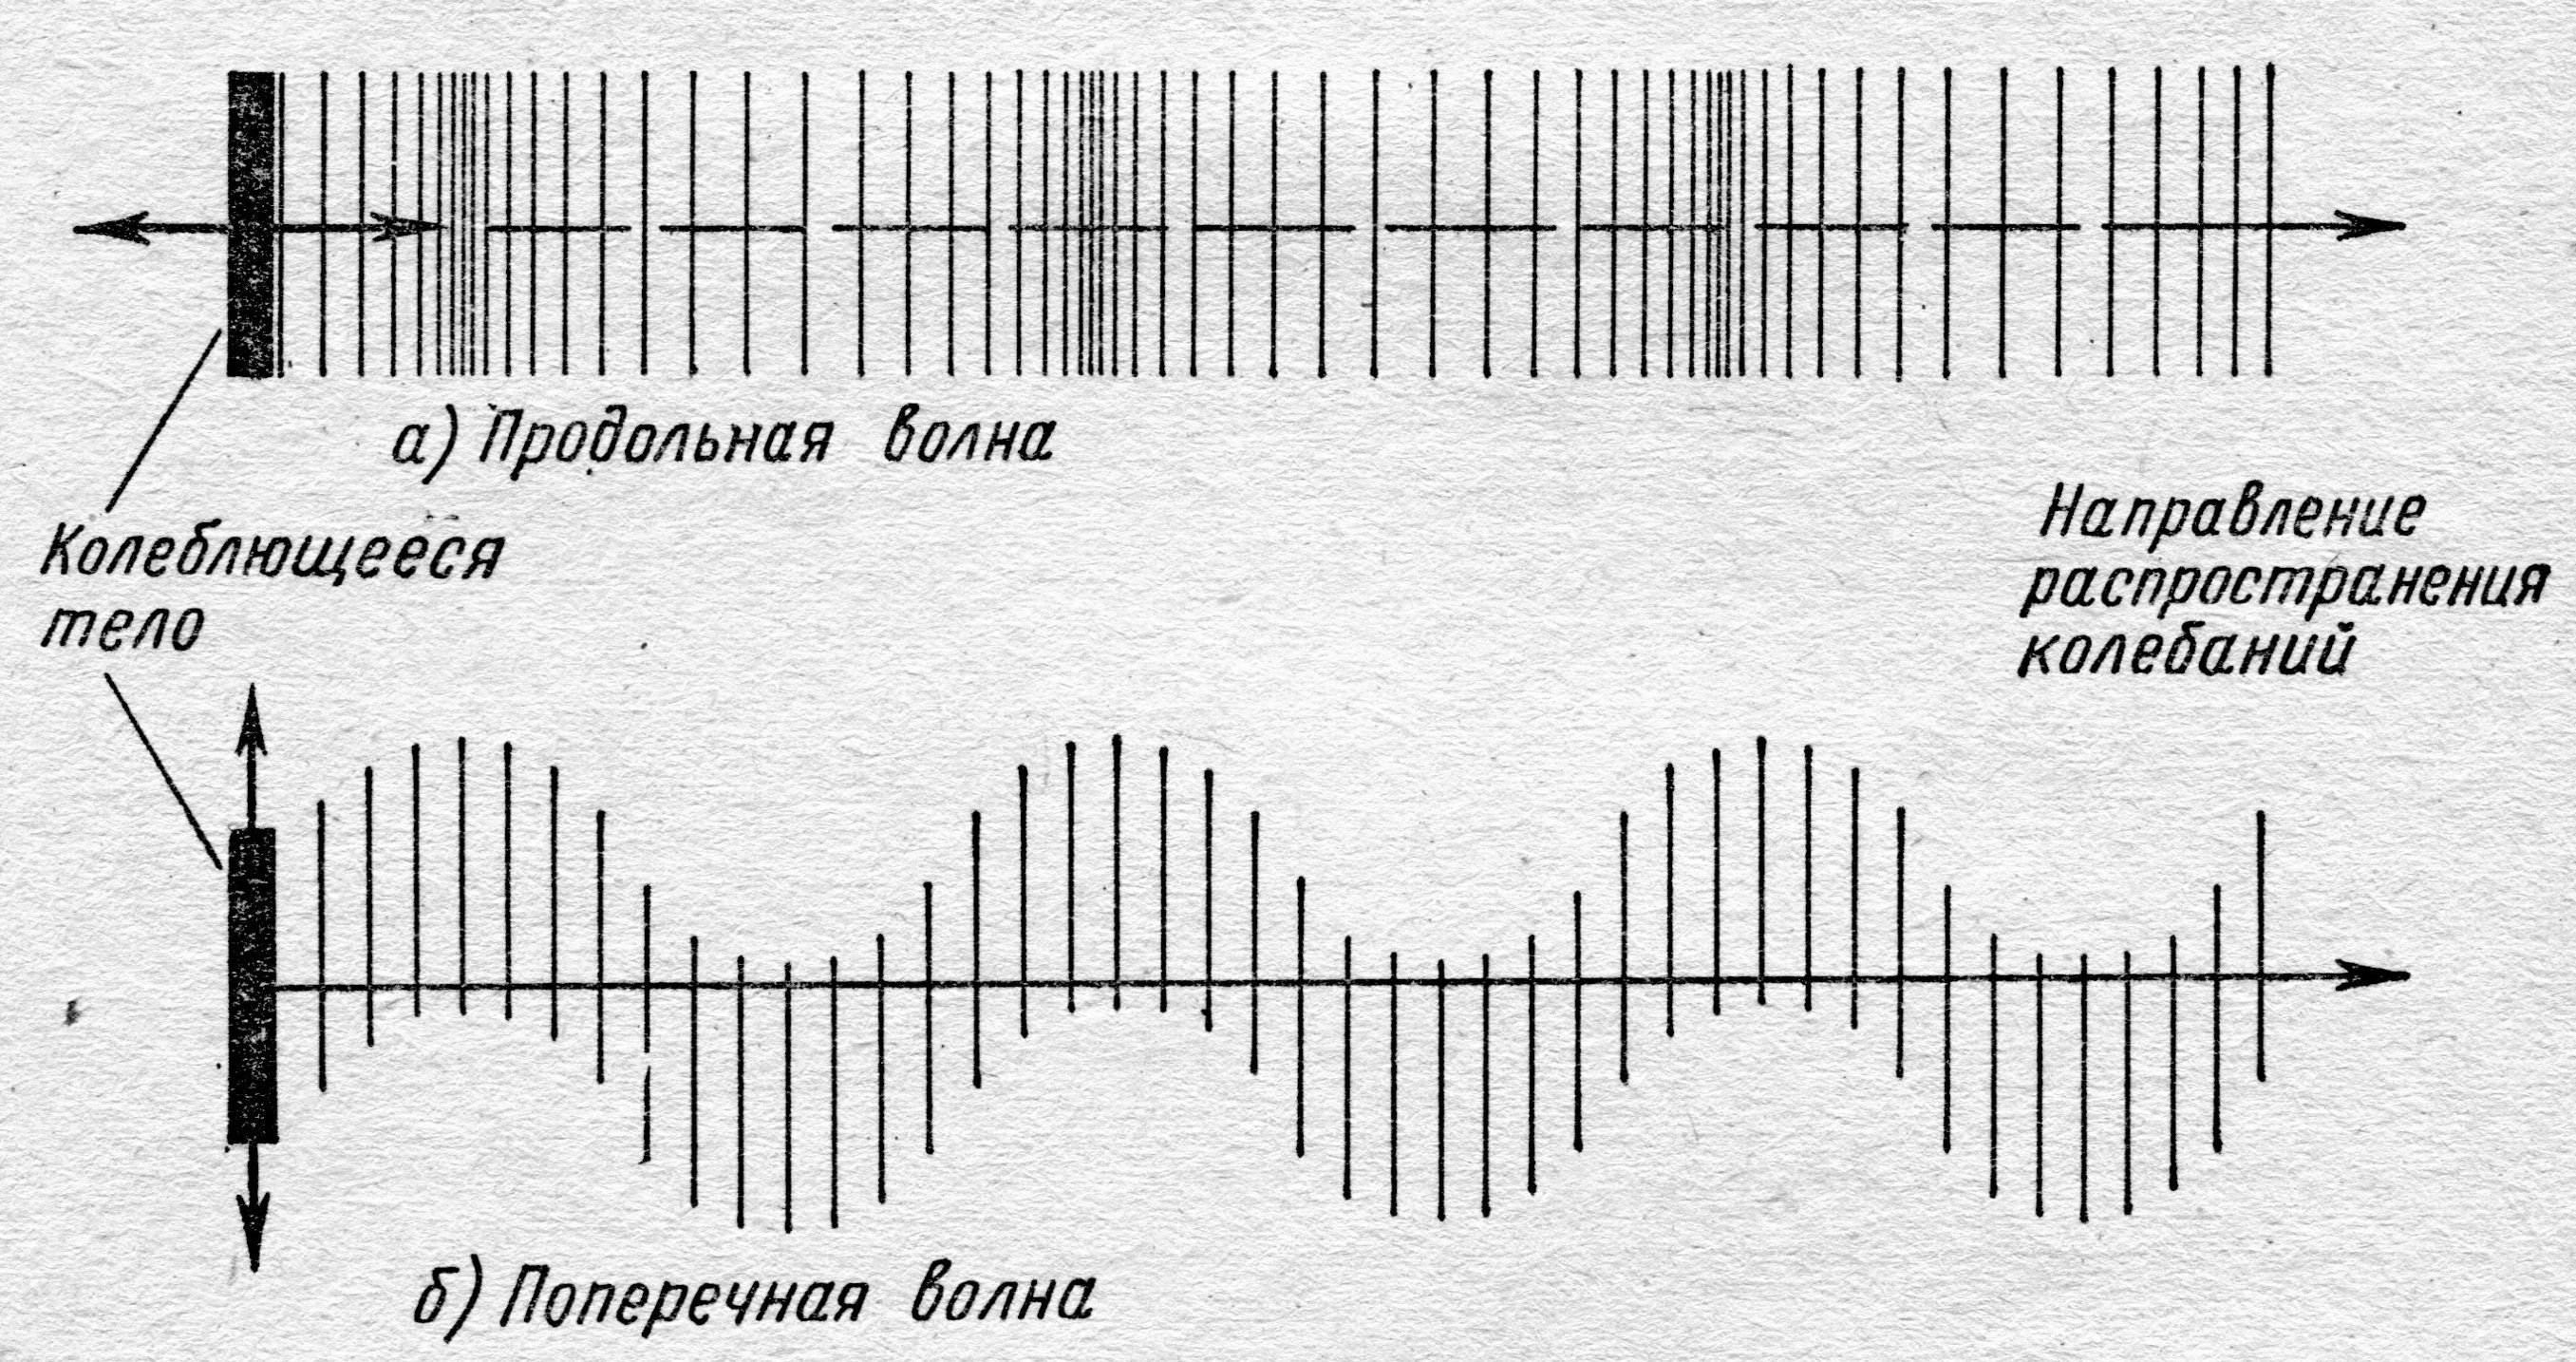
\includegraphics[width=0.75\textwidth]{physics2/images/physics2_2025_03_31_1}
\end{center}

\smallvspace

Аргумент косинус называется фазой $\varphi = \omega t - kx + \varphi_0$

Если зафиксировать значение фазы $\omega t - kx + \varphi_0 = \operatorname{const}$, то это значение с течением
времени перемещается в направлении оси $Ox$ со скоростью, определяемой из условия $\frac{d\varphi}{dt} = \frac{d}{dt} (\omega t - kx + \varphi_0) = 0$

Фронт волны -- это совокупность точек, колеблющихся в одной фазе, до которых в данный момент времени дошел волновой процесс

Волновая поверхность -- поверхность, проведенная через равновесные положения частиц среды, совершающих колебания в одинаковой фазе

Скорость многих механических волн может быть записана в общем виде: 

$v = \sqrt{\frac{\text{возвращающая сила, стремящаяся вернуть систему в состояние равновесия}}{\text{инерция системы, противодействующая этому переходу}}}$

\mediumvspace

Поток энергии - количество энергии, переносимое волной через определенную поверхность за единицу времени: $\Phi = \frac{dW}{dt}$ 

Плотность потока энергии - поток энергии через единичную площадку, перпендикулярную направлению волны: $J = \frac{d\Phi}{dS}$



% end physics2_2025_03_31.tex

% begin physics2_2025_04_07.tex





\section{Лекция 9. Интерференция света}

Поляризация света - упорядоченность в ориентации векторов напряженностей электрического поля $E$
и магнитного поля $H$ световой волны в плоскости, перпендикулярной распространению света

Различают: 

\begin{enumerate}
    \item линейную поляризацию света, когда ориентация вектора $E$ сохраняет постоянное направление 
(плоскость, в которой лежит $E$ и световой луч, называются плоскостью поляризации)

    \item эллиптическую поляризацию, при которой конец $E$ в проекции на плоскость, 
    перпендикулярную направлению света, описывает эллипс 

    \item круговою поляризацию, при которой конец $E$ описывает круг
\end{enumerate}

Обычный, естественный свет, например, от солнца, хаотично поляризован - конец $E$ описывает хаотичные фигуры

Интерференция света - нелинейное сложение интенсивностей двух или нескольких световых волн, 
сопровождающееся пространственным перераспределением энергии светового излучения

Если через точку проходят две волны с векторами $\vec E_1$ и $\vec E_2$, то в точке напряженность равна $E = E_1 + E_2$, 
а интенсивность света определяется так: $\langle \vec E^2 \rangle = \langle \vec E_1^2 \rangle + \langle \vec E_2^2 \rangle + 2\langle (\vec E^2_1, \vec E_2^2) \rangle$

Если $2\langle (\vec E^2_1, \vec E_2^2) \rangle = 0$, то интерференции нет, если $2\langle (\vec E^2_1, \vec E_2^2) \rangle \neq 0$, то есть 

В частности, если $E_1 \perp E_2$, то интерференции нет 

При этом интенсивность света в точке равна $I = I_1 + I_2 + 2\sqrt{I_1 I_2} \cos \langle \delta \rangle$, где $\langle \delta \rangle$ - разность фаз

Нарушение аддитивности интенсивности связано не с нарушением ЗСЭ, а с перераспределением энергии 
по волновому фронту при взаимодействии волн

Если разность фаз колебаний в точке постоянна, то есть $\langle \delta \rangle = \delta (r_1, r_2)$, то колебания и волны называют когерентными

Чтобы две световые синусоидальные волны были когерентными, их частоты должны быть одинаковыми.
Слагаемое $2\sqrt{I_1 I_2} \cos \langle \delta \rangle$ называют интерференционным членом

\mediumvspace

Рассмотрим два точечным источника света, которые описывают интерференционную картину на экране

\smallvspace

% https://www.geogebra.org/calculator/cbg9buf2

\begin{center}
    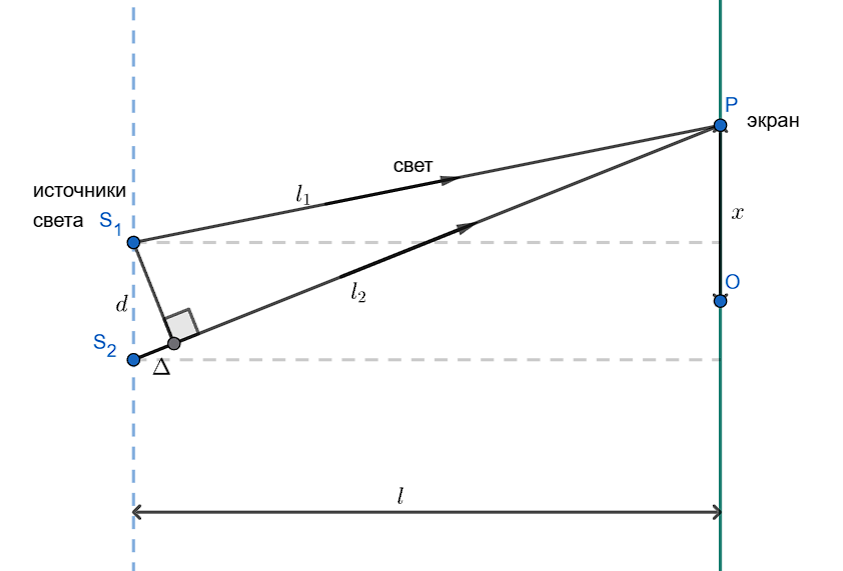
\includegraphics[width=0.75\textwidth]{physics2/images/physics2_2025_04_07_1}
\end{center}

\smallvspace

Величина $l = ns$, где $n$ - показатель преломления, называется оптической длиной пути, 
величина $\Delta \equiv l_1 - l_2$ - оптической разностью пути

Если $\Delta = n \frac{x d}{l} = m \lambda_0$ ($m \in \Integer$), то $\cos \delta = \cos 2\pi m = 1$, свет будет в одной фазе 
и в точке будет наблюдаться максимум интенсивности

А если $\Delta = \frac{2m + 1}{2} \lambda_0$, то будет наблюдаться минимум

В общем, на экране будет наблюдаться картина, состоящая из темных и светлых полос. Светлые полосы отображают
максимумы, а темные - минимумы

Если свет пропустить через решетку с тоненькими прорезями, то излучаемый оттуда свет можно считать точечными источникам.
И на экране получается картина из светлых и темных полос. Явление света огибать решетку получило название дифракция


% end physics2_2025_04_07.tex

% begin physics2_2025_04_14.tex





\section{Лекция 10. Интерференция в разных опытах}

\subsection{Оптическая разность хода и разность фаз}

Чтобы наблюдать интерференцию света, необходимо использовать когерентные источники, т.е. источники с постоянной разностью фаз. Получить два совершенно одинаковых независимых источника практически невозможно, поэтому используют один источник и делят его волновой фронт -- например, с помощью двух щелей. В этом случае два полученных пучка будут когерентными.

Важно понимать, что сама по себе оптическая разность хода между лучами не гарантирует интерференции. Для наблюдения интерференционной картины необходимо, чтобы лучи пересекались в пространстве и накладывались друг на друга. Если лучи в дальнейшем не пересекаются, интерференционные эффекты в этих областях не наблюдаются, даже несмотря на существование фиксированной разности хода.

\textbf{Оптическая разность хода} $\Delta$ -- это разность между произведениями геометрических длин путей, пройденных волнами, и показателей преломления сред, через которые проходят волны. Иначе говоря, она показывает, насколько одна волна \enquote{отстаёт} от другой по фазе из-за различий в длине пути и/или свойствах среды.

Если волна проходит путь $S$ в среде с показателем преломления $n$, её фаза:
\[
\varphi = \omega t - k S + \varphi_0 = \omega t - \frac{2\pi n}{\lambda_0} S + \varphi_0
\]

Для двух лучей разность фаз будет:
\[
\Delta = \varphi_2 - \varphi_1 = \frac{2\pi}{\lambda_0}(n_1 S_1 - n_2 S_2)
\]

Алгоритм вычисления оптической разности хода:
\begin{enumerate}
  \item Определить пути $S_1$ и $S_2$, пройденные волнами.
  \item Определить показатели преломления $n_1$ и $n_2$ сред, через которые проходят волны.
  \item Вычислить: \[ \Delta = n_1 S_1 - n_2 S_2. \]
  \item Если волны идут по воздуху ($n_1 = n_2 = 1$), формула упрощается до разности геометрических длин.
\end{enumerate}


\subsection{Интерференционные полосы (опыт Юнга)}

Томас Юнг в своём знаменитом эксперименте использовал одну щель как источник света, проходящего через две узкие щели. На экране за ними возникала интерференционная картина -- чередующиеся светлые и тёмные полосы.

Пусть расстояние между щелями $d$, расстояние до экрана $L$, а $x$ -- поперечная координата на экране:
\[
\Delta = d \sin \theta \approx \frac{d x}{L}, \quad \text{где } x \text{ --- координата полосы}
\]

Для максимумов интерференции:
\[
\Delta = m\lambda \Rightarrow x_m = \frac{m\lambda L}{d}
\]

\subsection{Призма}

При прохождении света через тонкую призму с углом преломления $\alpha$ и показателем преломления $n$:
\[
\alpha_1 = n\beta_1, \quad \alpha_2 = n\beta_2, \quad \beta_1 + \beta_2 = \alpha
\]

Итоговая разность хода:
\[
\Delta = (\alpha_1 + \alpha_2) - (\beta_1 + \beta_2) = n\alpha - \alpha = \alpha(n - 1)
\]

\subsection{Билинза Френеля}

Это приспособление, создающее два когерентных пучка с помощью симметрично расположенных линз. Оптическая разность хода:
\[
\Delta = 2\alpha(n - 1)a
\]

Если $a + b = L$, где $b$ -- расстояние от билинзы до экрана, то координаты интерференционных максимумов:
\[
x_m = m \frac{l}{d} \lambda = m \frac{a + b}{2 \alpha (n - 1) a} \lambda
\]
Для центрального максимума ($m = 0$), центр находится в точке:
\[
x_0 = \frac{b}{2 \alpha (n - 1)}
\]


\subsection{Интерференция от полупрозрачного зеркала}

При отражении света от границы между двумя средами, если свет отражается от более оптически плотной среды (с большим показателем преломления), то он приобретает сдвиг фазы на $\frac{\lambda}{2}$. Это означает, что волна, отразившаяся от более плотной среды, будет иметь фазовый сдвиг относительно той, которая прошла через границу.

\[
\Delta = a - b + \frac{\lambda}{2}
\]

\subsection{Интерференция в тонкой пластине}

Свет частично отражается от верхней и нижней поверхностей тонкой плёнки с показателем преломления $n$. Разность хода:
\[
\sin \alpha = n \sin \gamma
\]

\[
\Delta = 2nh\cos \gamma = \frac{2nh}{\sqrt{1 - \frac{\sin^2 \alpha}{n^2}}}
\]

\subsection{Клиновидная пластина}

\textbf{Клиновидная пластина} -- тонкий слой материала с переменной толщиной, вызывает интерференцию с переменной разностью хода, что приводит к чередованию полос. Разность хода в этом случае будет:
\[
\Delta(x) = 2n x \tan \theta
\]

Положение тёмных полос определяется условием разрушительной интерференции:
\[
\x_m = \frac{(2m + 1)\lambda}{4n \tan \theta}
\]

\subsection{Кольца Ньютона}

\textbf{Кольца Ньютона} -- интерференционная картина, возникающая при наложении выпуклой линзы на плоскую пластину. Возникают концентрические кольца из-за различной толщины воздушного зазора $h(r)$:
\[
h(r) = \frac{r^2}{2R} \Rightarrow \Delta = 2n h = \frac{n r^2}{R}
\]

Для тёмных колец:
\[
\frac{n r_m^2}{R} = (2m + 1)\frac{\lambda}{2} \Rightarrow r_m = \sqrt{\frac{(2m + 1)\lambda R}{2n}}
\]

\subsection{Дифракция света}

Дифракция -- явление огибания светом препятствий, не объяснимое законами геометрической оптики. Свидетельствует о волновой природе света и проявляется, например, в виде характерных полос за узкими щелями и объектами.

Типичные примеры:
\begin{itemize}
  \item дифракция на щели;
  \item дифракция на проволоке;
  \item дифракция Фраунгофера и Френеля.
\end{itemize}

\textbf{Условие минимума при дифракции на щели:} $a \sin \theta = m \lambda, \quad m \in \mathbb{Z}$, где $a$ -- ширина щели.

\textbf{Условие максимума при дифракции на щели:} $d \sin \theta = m \lambda, \quad m \in \mathbb{Z}$, где $d$ -- период решетки (ширина щели + ширина препятствия).

Или $a \sin \theta = \frac{1}{2} (2m + 1) \lambda, \quad m \in \mathbb{Z}$

% end physics2_2025_04_14.tex

% begin physics2_2025_04_21.tex





\section{Лекция 11. Дифракция}

Дифракция в оптике — это совокупность явлений, связанных с отклонением света от прямолинейного пути распространения. Особенно ярко дифракционные эффекты проявляются при прохождении света мимо непрозрачных препятствий, хотя дифракция может возникать и при взаимодействии света с прозрачными объектами. В узком смысле дифракция — это огибание волнами препятствий, что характерно для всех типов волн, включая световые.

Принцип Гюйгенса утверждает: каждая точка среды, до которой дошла волна, становится источником вторичных сферических волн. Огибающая этих волн определяет форму волнового фронта в следующий момент времени.

Френель развил этот принцип, сделав его более количественным и применимым к объяснению дифракции:
\begin{itemize}
  \item Все вторичные источники на волновом фронте когерентны между собой, если исходная волна была когерентной.
  \item Равные по площади участки фронта излучают равные по мощности вторичные волны.
  \item Излучение каждого вторичного источника направлено преимущественно вдоль нормали к фронту.
  \item Действует принцип суперпозиции: волны от разных участков фронта складываются независимо. Если часть фронта экранируется, остальные участки продолжают излучать, как если бы экрана не было.
\end{itemize}

На основе этих положений формулируется принцип Гюйгенса–Френеля: каждый элемент волнового фронта можно рассматривать как центр вторичного возмущения, излучающего сферические волны. Амплитуда в некоторой точке $P$ определяется суперпозицией всех таких волн.

Амплитуда сферической волны, приходящей в точку $P$ от малого элемента поверхности $\Delta S$, зависит от расстояния $r$ до точки $P$, угла $\theta$ между нормалью к $\Delta S$ и направлением $r$, и пропорциональна $\Delta S$:
\[ E_P = \int_S K(\theta) \frac{E_0}{r} \cos(kr + \varphi_0)\, dS \]

Здесь $K(\theta)$ — коэффициент, зависящий от угла, $k = \frac{2\pi}{\lambda}$ — волновое число, $E_0$ — амплитуда первичной волны, $\varphi_0$ — её начальная фаза.

Дифракция Френеля — это дифракция сферических волн, когда источник и экран находятся на конечном расстоянии. Если же свет представлен параллельными пучками, и источник и экран расположены на бесконечности (или фокусируются линзой), говорят о дифракции Фраунгофера.

Волновая поверхность сферической волны симметрична относительно оси $SP$. Френель предложил разбивать волновую поверхность на шаровые зоны так, чтобы разность хода между волнами от границ соседних зон была равна $\lambda/2$. Вклад от каждой последующей зоны идёт с чередующейся фазой, и суммарная амплитуда зависит от числа таких зон.

Рассмотрим дифракцию плоской волны на бесконечно длинную щель шириной $b$. Пусть плоская волна падает на щель под углом $\theta$. Тогда оптическая разность хода между волнами, идущими от противоположных краёв щели, будет:
\[ \Delta = b \sin \theta \]

Если $\Delta = k\frac{\lambda}{2}$, где $k$ — целое число, то волны от краёв щели интерферируют, и картина зависит от того, сколько зон Френеля укладывается в ширину щели:
\begin{itemize}
  \item если число зон чётное — волны взаимно гасятся, и в точке наблюдается минимум;
  \item если число зон нечётное — центральная зона не компенсирована, и наблюдается максимум.
\end{itemize}

В направлении $\theta = 0$ вся щель действует как одна зона Френеля. Это даёт центральный максимум — он самый яркий и широкий.

% end physics2_2025_04_21.tex

% begin physics2_2025_04_28.tex





\section{Лекция 12. Дифракция и поляризация}

\subsection{Дифракция на системе щелей}

Дифракционная решётка состоит из большого числа одинаковых щелей, разделённых непрозрачными промежутками. Дифракционные картины, создаваемые каждой щелью, совпадают по виду и интерферируют друг с другом. Суммарная картина наблюдается как результат интерференции когерентных волн, выходящих из всех щелей решётки.

Пусть ширина каждой щели равна $b$, ширина непрозрачной прослойки между щелями — $a$. Тогда полный период решётки $d = a + b$. Это расстояние между центрами двух соседних щелей. Также $d = \frac{1}{N_0}$, где $N_0$ — число щелей на единицу длины решётки (пространственная плотность щелей).

Разность хода между волнами, идущими из двух соседних щелей под углом $\theta$ к нормали, равна:
\[
\Delta = d \sin \theta
\]

Условия наблюдения дифракционной картины:
\begin{itemize}
    \item \textbf{Главные максимумы (интерференционные пики)} наблюдаются, когда волны от всех $N$ щелей приходят в фазе:
    \[
    d \sin \theta = m \lambda, \quad m \in \mathbb{Z}
    \]
    
    \item \textbf{Главные минимумы} для одной щели возникают, если края щели создают волны в противофазе:
    \[
    b \sin \theta = m \lambda
    \]
    
    Это определяет подавление интенсивности для каждой отдельной щели. При этом даже если выполняется условие максимума решётки, максимум может исчезнуть, если $\theta$ также соответствует минимуму одиночной щели.

    \item \textbf{Дополнительные минимумы} (между главными максимумами) появляются при:
    \[
    d \sin \theta = \left(2m + 1\right) \frac{\lambda}{2}
    \]
    Их физическая природа связана с частичной компенсацией амплитуд от разных щелей. Между каждыми двумя соседними главными максимумами находится $N - 1$ дополнительных минимума.
\end{itemize}

Интенсивность в направлении главного максимума в $N^2$ раз превышает интенсивность от одной щели:
\[
I_{\max} = N^2 I_1
\]
где $I_1$ — интенсивность от одной щели в направлении главного максимума. Это происходит потому, что амплитуды складываются:
\[
A_{\max} = N A_1
\Rightarrow I \propto A^2
\]

Фазовые сдвиги при интерференции можно учесть, считая колебания от первой щели:
\[
A_1(t) = A_0 \cos \omega t
\]
От второй щели:
\[
A_2(t) = A_0 \cos(\omega t - \Delta \varphi)
\]
От $k$-й щели:
\[
A_k(t) = A_0 \cos\left(\omega t - (k - 1)\Delta \varphi\right)
\]

Эти колебания можно представить как сумму комплексных экспонент:
\[
\sum_{k=1}^N A_0 e^{i(\omega t - (k - 1)\Delta \varphi)} = A_0 e^{i\omega t} \sum_{k=0}^{N-1} e^{-i k \Delta \varphi}
\]

Это конечная геометрическая прогрессия, которая может быть просуммирована. Таким образом можно получить зависимость амплитуды и интенсивности от угла $\theta$.

Центральный (нулевой) максимум наблюдается при $\theta = 0$ и не зависит от длины волны $\lambda$. Поэтому он содержит все длины волн и выглядит белым на экране при освещении белым светом.


\subsection{Поляризация света}

Свет — это электромагнитная волна, в которой переменные электрическое и магнитное поля колеблются перпендикулярно направлению распространения. При этом электрическое поле играет основную роль при взаимодействии с веществом, поэтому его направление называют направлением поляризации.

Если вектор электрического поля сохраняет своё направление при распространении, такая волна называется линейно или плоско-поляризованной. Поляризация — это проявление поперечной природы световых волн.

Поляризатор — это устройство, преобразующее неполяризованный свет в поляризованный. Анализатор — прибор, позволяющий проверить, поляризован ли свет.

Явление, при котором степень поглощения света зависит от направления колебаний электрического поля, называется дихроизмом. 

Поляроид — это полимерная плёнка, содержащая ориентированные кристаллы дихроичного вещества. Он пропускает колебания только в одном направлении и поглощает в перпендикулярном, эффективно действуя как поляризатор.

\textbf{Закон Малюса:}
Если на анализатор падает линейно-поляризованный свет, и угол между направлениями поляризации и пропускания анализатора равен $\varphi$, то:
\[
I = I_0 \cos^2 \varphi
\]
где $I_0$ — интенсивность падающего света, $I$ — интенсивность прошедшего через анализатор.

\textbf{Угол Брюстера:} при падении света на границу двух сред под некоторым углом, отражённый свет становится полностью поляризованным. Этот угол определяется из условия:
\[
\tan \theta_B = \frac{n_2}{n_1}
\]

\textbf{Формулы Френеля:} описывают амплитуды отражённых и преломлённых волн при падении под произвольным углом на границу двух диэлектриков. Они позволяют рассчитать степень поляризации отражённого света.

\textbf{Степень поляризации} света определяется как:
\[
P = \frac{I_{\max} - I_{\min}}{I_{\max} + I_{\min}}
\]
где $I_{\max}$ и $I_{\min}$ — максимальная и минимальная интенсивности при вращении анализатора.

\textbf{Эффект Керра:} в сильных электрических полях в некоторых веществах возникает искусственная двойная лучепреломляемость. Свет, проходящий через такое вещество, становится частично поляризованным.


% end physics2_2025_04_28.tex

% begin physics2_2025_05_05.tex





\section{Лекция 13. Модель атома}

Модель Томпсона представляла собой «пудинг с изюмом»: атом — это положительно заряженная сфера, внутри которой равномерно распределены отрицательные электроны. Такая модель могла объяснить нейтральность атома, но не допускала существования чёткой структуры внутри атома и не давала объяснения наблюдаемым спектрам.

Опыт Резерфорда (1911) стал поворотным моментом. Альфа-частицы (ядра гелия) направлялись на тонкую золотую фольгу. Большинство частиц проходило без отклонения, но некоторые отклонялись на большие углы, а отдельные — почти обратно. Это можно объяснить только в предположении, что в центре атома сосредоточен положительный заряд и почти вся масса — то есть существует ядро. Модель Томпсона не может это объяснить: в ней нет плотного центра, который мог бы отклонить тяжёлую альфа-частицу.

Так появилась модель Резерфорда: атом состоит из тяжёлого положительно заряженного ядра, вокруг которого по орбитам движутся электроны, как планеты вокруг Солнца. Но классическая электродинамика предсказывает, что ускоренно движущийся электрон должен излучать энергию, терять её и, за долю секунды, упасть на ядро. Это противоречит стабильности атомов.

Чтобы объяснить устойчивость атома и его спектры, Нильс Бор в 1913 году предложил свою модель. Он ввёл постулаты:

\begin{enumerate}
    \item Электрон может двигаться по стационарной орбите без излучения.
    \item Излучение или поглощение происходит при переходе между орбитами.
    \item Угловой момент электрона на орбите квантован:
    \[
    L = m v r = n \hbar, \quad n \in \mathbb{N}
    \]
\end{enumerate}

Для наименьшей орбиты (основное состояние, $n = 1$) получим радиус Бора:
\[
r_n = \frac{n^2 \hbar^2}{m k e^2} = n^2 r_1, \quad r_1 \approx 5.29 \cdot 10^{-11} \text{ м}
\]

Здесь $k = \frac{1}{4\pi\varepsilon_0}$ — коэффициент из закона Кулона.

Полная энергия электрона в $n$-й орбите:
\[
E_n = - \frac{m e^4}{2 \hbar^2 n^2 (4 \pi \varepsilon_0)^2} = -\frac{13.6\ \text{эВ}}{n^2}
\]

При переходе с уровня $n_2$ на $n_1$ (где $n_2 > n_1$), излучается фотон энергии:
\[
h \nu = E_{n_2} - E_{n_1}
\]

Эта формула объясняет спектральные линии водорода.

Постоянная Ридберга — это универсальная константа в формулах для спектров:
\[
\frac{1}{\lambda} = R \left( \frac{1}{n_1^2} - \frac{1}{n_2^2} \right), \quad R \approx 1.097 \cdot 10^7\ \text{м}^{-1}
\]

Серии в спектре водорода:

\begin{itemize}
    \item серия Лаймана: $n_1 = 1$, $n_2 = 2, 3, \ldots$ (ультрафиолет)  
    \item серия Бальмера: $n_1 = 2$, $n_2 = 3, 4, \ldots$ (видимый диапазон)  
    \item серия Пашена: $n_1 = 3$, $n_2 = 4, 5, \ldots$ (инфракрасный диапазон)
\end{itemize}

Состояние атома, в котором электрон находится на орбите с минимально возможной энергией, называется \textbf{основным}. Все остальные орбиты соответствуют \textbf{возбуждённым} состояниям. Атом может находиться в возбуждённом состоянии конечное время, после чего спонтанно переходит в основное, испуская фотон.

Опыт Франка и Герца (1914) экспериментально подтвердил существование дискретных энергетических уровней в атоме. Электроны ускорялись и сталкивались с атомами. При достижении определённой энергии (около 4.9 эВ для ртути), электроны теряли энергию, возбуждая атомы. Это означало, что атомы могут поглощать энергию только порциями — квантуемыми значениями, — соответствующими разности уровней.

Термин \textbf{электронное облако} — это современное представление о распределении вероятности нахождения электрона в атоме. Оно заменяет точечное положение орбиты и говорит о том, где с большей вероятностью можно найти электрон. Это уже относится к квантово-механической модели атома, основанной на уравнении Шрёдингера, а не на модели Бора.

Сила Ван-дер-Ваальса — это слабое взаимодействие между нейтральными атомами и молекулами, обусловленное флуктуациями электронных оболочек. Это не имеет прямого отношения к атомным моделям, но важно для понимания межмолекулярных взаимодействий.

% end physics2_2025_05_05.tex

% begin physics2_2025_05_12.tex





\section{Лекция 14. Уравнение Шрёдингера}

Свет проявляет как волновые, так и корпускулярные свойства. Эта дуалистическая природа описывается следующими соотношениями:

\[
E = \hbar \omega, \quad \abs{\vec{p}} = \hbar \abs{\vec{k}} = \frac{2\pi \hbar}{\lambda} = \frac{h}{\lambda}
\]

Здесь $E$ — энергия, $\omega$ — угловая частота, $\vec{p}$ — импульс, $\vec{k}$ — волновой вектор, $\lambda$ — длина волны, $h = 6.626 \cdot 10^{-34} \text{ Дж}\cdot\text{c}$ — постоянная Планка, $\hbar = \frac{h}{2\pi}$.

Луи де Бройль предположил, что если свет обладает как волновыми, так и корпускулярными свойствами, то подобный дуализм должен быть присущ и обычной материи: электронам, протонам и другим частицам. Он ввёл понятие волны, соответствующей частице. Её длина определяется соотношением:

\[
\lambda = \frac{h}{p}
\]

а частота:

\[
\omega = \frac{E}{\hbar}
\]

где $p$ — импульс частицы, $E$ — её энергия. Для свободной частицы с массой $m$ и без потенциальной энергии:

\[
E = \frac{p^2}{2m}
\]

Таким образом, даже электрону можно сопоставить волну, и он может проявлять интерференцию и дифракцию. Это было экспериментально подтверждено.

\textbf{Опыт Дэвиссона и Джермера (1927):} при прохождении пучка электронов через кристалл никеля была обнаружена дифракционная картина, аналогичная картине от рентгеновского излучения. Это стало доказательством волновых свойств электронов.

\textbf{Электрон как облако вероятностей:} из-за волновой природы частицы нельзя точно указать её положение и импульс одновременно. Электрон описывается не как точечный объект, а как облако вероятностей, где выше вероятность нахождения — там выше $|\psi|^2$.

\textbf{Принцип неопределённости Гейзенберга:}

\[
\Delta x \cdot \Delta p \gtrsim \frac{\hbar}{2}
\]

где $\Delta x$ — неопределённость координаты, $\Delta p$ — неопределённость импульса. Это фундаментальное ограничение, вытекающее из самой природы квантовых объектов.

\textbf{Волновая функция $\psi(\vec{r}, t)$} — центральное понятие квантовой механики. Её квадрат модуля $|\psi|^2$ показывает вероятность обнаружить частицу в данной точке пространства в данный момент времени. Волновая функция может быть комплексной, но физически измеримыми являются только производные от неё величины.

\textbf{Уравнение Шрёдингера} описывает эволюцию волновой функции. Оно заменяет законы Ньютона в квантовом мире:

\[
i\hbar \frac{\partial \psi(\vec{r}, t)}{\partial t} = \hat{H} \psi(\vec{r}, t)
\]

Здесь $\hat{H}$ — гамильтониан — оператор полной энергии. Он состоит из оператора кинетической энергии и потенциальной:

\[
\hat{H} = -\frac{\hbar^2}{2m} \nabla^2 + V(\vec{r})
\]

Первая часть — кинетическая энергия, выраженная через оператор Лапласа, вторая — потенциальная энергия $V(\vec{r})$.

Таким образом, уравнение Шрёдингера показывает, как изменяется волновая функция во времени под действием полной энергии системы.

\textbf{Стационарное уравнение Шрёдингера} (если потенциал не зависит от времени):

\[
\hat{H} \psi(\vec{r}) = E \psi(\vec{r})
\]

Это уравнение на собственные значения: мы ищем такие функции $\psi$, при которых действие оператора $\hat{H}$ приводит к умножению на число $E$ — энергию.

\textbf{Свойства волновой функции:}
\begin{itemize}
    \item $\psi$ должна быть нормируемой: $\int |\psi|^2 dV = 1$
    \item должна быть конечной, непрерывной и однозначной во всех точках
    \item производные $\psi$ также должны быть непрерывными (кроме точек, где потенциал имеет особые особенности)
\end{itemize}

Всё поведение микрочастиц в квантовой механике может быть выведено из уравнения Шрёдингера, что делает его фундаментом современной теоретической физики.

% end physics2_2025_05_12.tex

% begin physics2_exam_list.tex
\clearpage

\section{X. Программа экзамена в 2024/2025}

\begin{enumerate}

    \item Гармонический осциллятор. Уравнение гармонических колебаний. Энергия гармонических колебаний. Примеры механических колебаний: пружинный и математический маятник. Физический маятник. Частота, круговая частота и период колебаний. Фазовый портрет маятника. Адиабатические инварианты.

    \item Затухающие механические колебания. Анализ затухающих колебаний. Сухое и вязкое трение. Коэффициент затухания, логарифмический декремент затухания, добротность.

    \item Вынужденные колебания. Колебания материальной точки под действием вынуждающей синусоидальной силы. Резонанс. Резонансные кривые. Параметрический резонанс.

    \item Сложение колебаний. Биения. Моды колебаний связанных математических маятников.

    \item Волны: волновое уравнение, свойства решений волнового уравнения, основные понятия - волновой вектор, длина волны, фазовая скорость. Продольные и поперечные волны. Плоские и сферические волны.

    \item Вывод уравнения электромагнитных (эл/м) волн из уравнений Максвелла.

    \item Свойства эл/м волн (поперечность, связь электрического и магнитного полей, синфазность колебаний электрического и магнитного полей).

    \item Плотность потока энергии в эл/м волне (вектор Пойтинга).

    \item Условия интерференции. Интерференция монохроматических световых волн. Двухлучевая интерференция: схема опыта Юнга, интерференционные схемы.

    \item Интерференция в тонких пленках. Кольца Ньютона.

    \item Принцип Гюйгенса-Френеля (определение и математическая формулировка).

    \item Дифракция Френеля на круглом отверстии: зоны Френеля, спираль Френеля, пятно Пуассона.

    \item Режимы дифракции (Френеля, Фраунгофера).

    \item Дифракция Фраунгофера на щели, свойства дифракционной картины.

    \item Дифракционная решетка в монохроматическом свете, свойства дифракционной картины.

    \item Дифракционная решетка как спектральный прибор: угловая дисперсия при дифракции на решетке, разрешающая способность дифракционной решетки.

    \item Поляризованный и естественный свет, линейная и круговая поляризации, закон Малюса, степень поляризации.

    \item Законы отражения и преломления э/м волн.

    \item Поляризация при отражении и преломлении: формулы Френеля.

    \item Применение формул Френеля: угол Брюстера, скачок фазы при отражении, коэффициент отражения.

    \item Основы кристаллооптики: тензор диэлектрической проницаемости, уравнение распространения плоской волны в анизотропной среде.

    \item Двулучепреломление: основные понятия, одноосные и двуосные кристаллы, поляризаторы (призма Николя, призма Фуко, поляроиды), фазовые пластинки (λ/4 и λ/2).
\end{enumerate}

% end physics2_exam_list.tex



\end{document}

